\begin{English}
\section{Hardware}
\end{English}

\begin{Czech}
\section{Hardware}
\end{Czech}

% ====================  START Central Control Unit ====================
\begin{English}
\subsection{The Central Unit}
\end{English}

\begin{Czech}
\subsection{Centrální jednotka}
\end{Czech}


\begin{English}
In the figure \ref{fig:central-control-unit-case-top}, there is the central unit with a description of individual LEDs a switches.
\end{English}

\begin{Czech}
Na obrázku \ref{fig:central-control-unit-case-top} je centrální jednotka s popisem jednotlivých LED a přepínačů.
\end{Czech}


\begin{English}
\begin{figure}[H]
\centering
\begin{tikzpicture}[font=\sffamily]
     \node[anchor=south west,inner sep=0] (image) at (0,0) {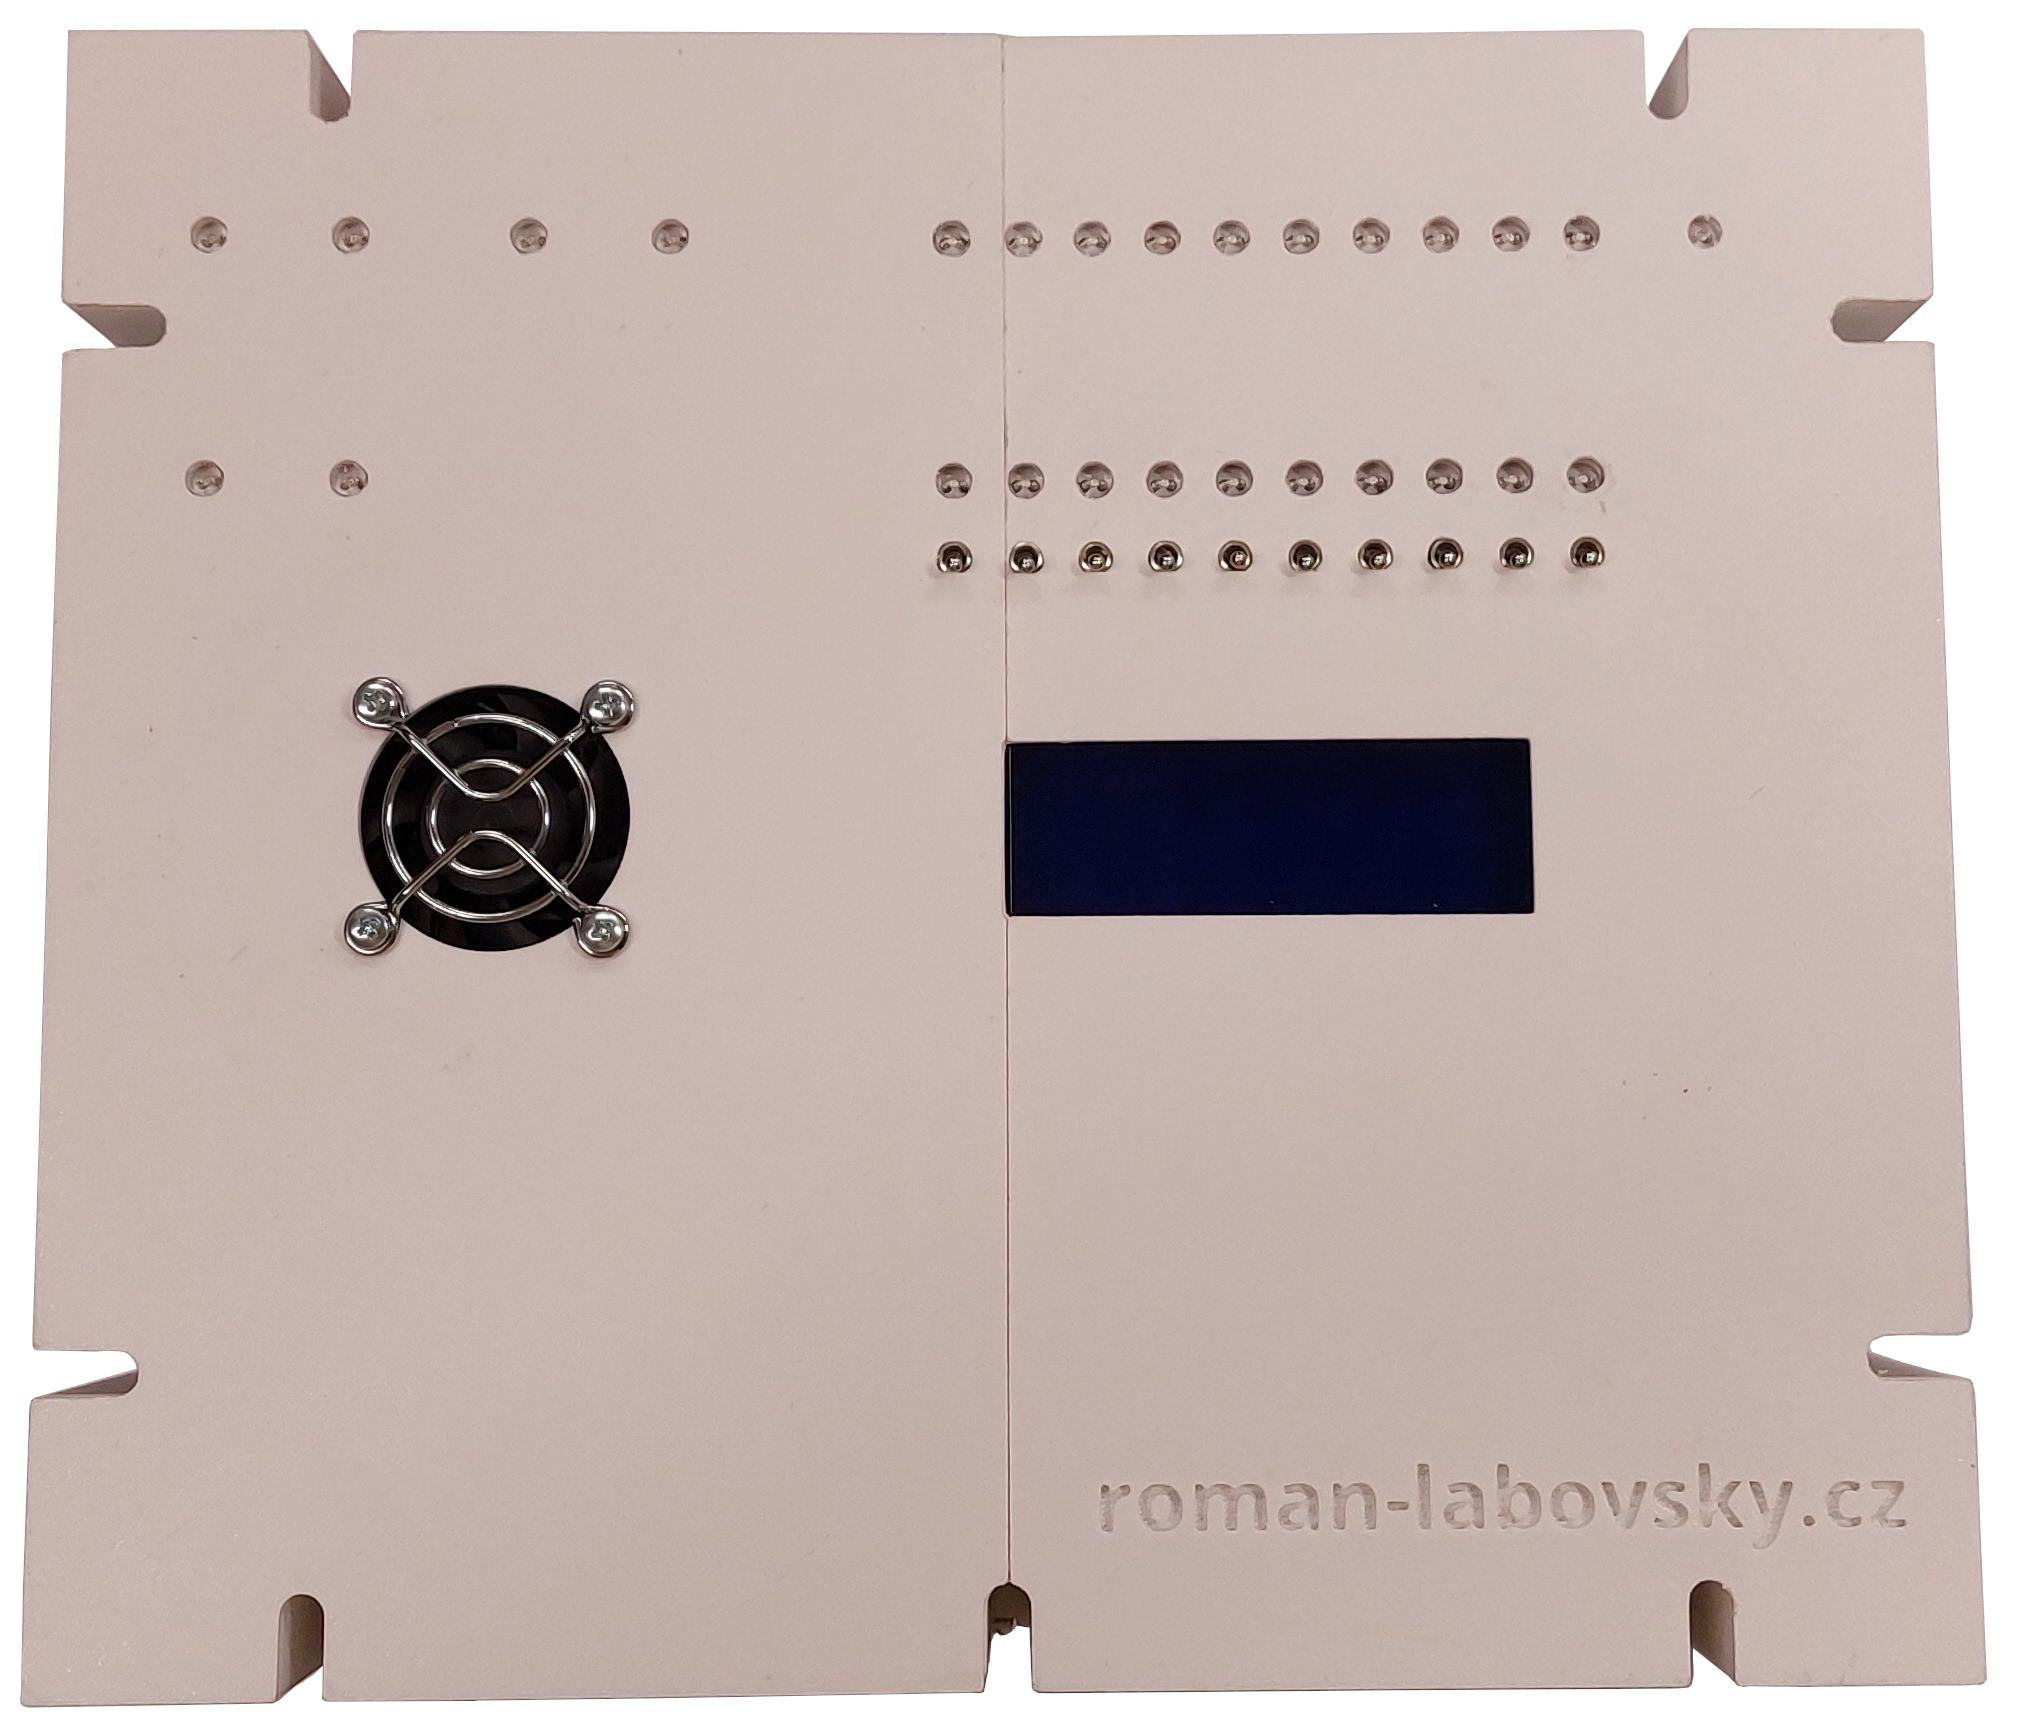
\includegraphics[width=1\textwidth]{pictures/all/hardware/central-control-unit-case-top.jpg}};
      \begin{scope}[x={(image.south east)},y={(image.north west)}]
     	% start SUPPORT GRID
        %\draw[help lines,xstep=.1,ystep=.1] (0,0) grid (1,1);
        %\foreach \x in {0,1,...,9} { \node [anchor=north] at (\x/10,0) {0.\x}; }
        %\foreach \y in {0,1,...,9} { \node [anchor=east] at (0,\y/10) {0.\y}; }
     	% end SUPPORT GRID
                 
          \node[text=red] at (0.1,0.9) {1a};
          \node[text=red] at (0.1,0.76) {1b};
          
          \node[text=red] at (0.17,0.9) {2a};
          \node[text=red] at (0.17,0.76) {2b};
         
          \node[text=red] at (0.26,0.9) {3};
          \node[text=red] at (0.33,0.9) {4};
          
          \node[text=red] at (0.465,0.9) {5a};
          \node[text=red] at (0.505,0.9) {6a};
          \node[text=red] at (0.540,0.9) {7a};
          \node[text=red] at (0.575,0.9) {8a};
          \node[text=red] at (0.610,0.9) {9a};
          \node[text=red] at (0.645,0.9) {10a};
          
          \node[text=red] at (0.465,0.76) {5b};
          \node[text=red] at (0.505,0.76) {6b};
          \node[text=red] at (0.540,0.76) {7b};
          \node[text=red] at (0.575,0.76) {8b};
          \node[text=red] at (0.610,0.76) {9b};
          \node[text=red] at (0.645,0.76) {10b};
          
          \node[text=red] at (0.465,0.64) {5c};
          \node[text=red] at (0.505,0.64) {6c};
          \node[text=red] at (0.540,0.64) {7c};
          \node[text=red] at (0.575,0.64) {8c};
          \node[text=red] at (0.610,0.64) {9c};
          \node[text=red] at (0.645,0.64) {10c};
          
          \node[text=red] at (0.84,0.9) {11};
        \end{scope}
\end{tikzpicture}
\caption{The central unit with a cover.}
\label{fig:central-control-unit-case-top}
\end{figure}
\end{English}

\begin{Czech}
\begin{figure}[H]
\centering
\begin{tikzpicture}[font=\sffamily]
     \node[anchor=south west,inner sep=0] (image) at (0,0) {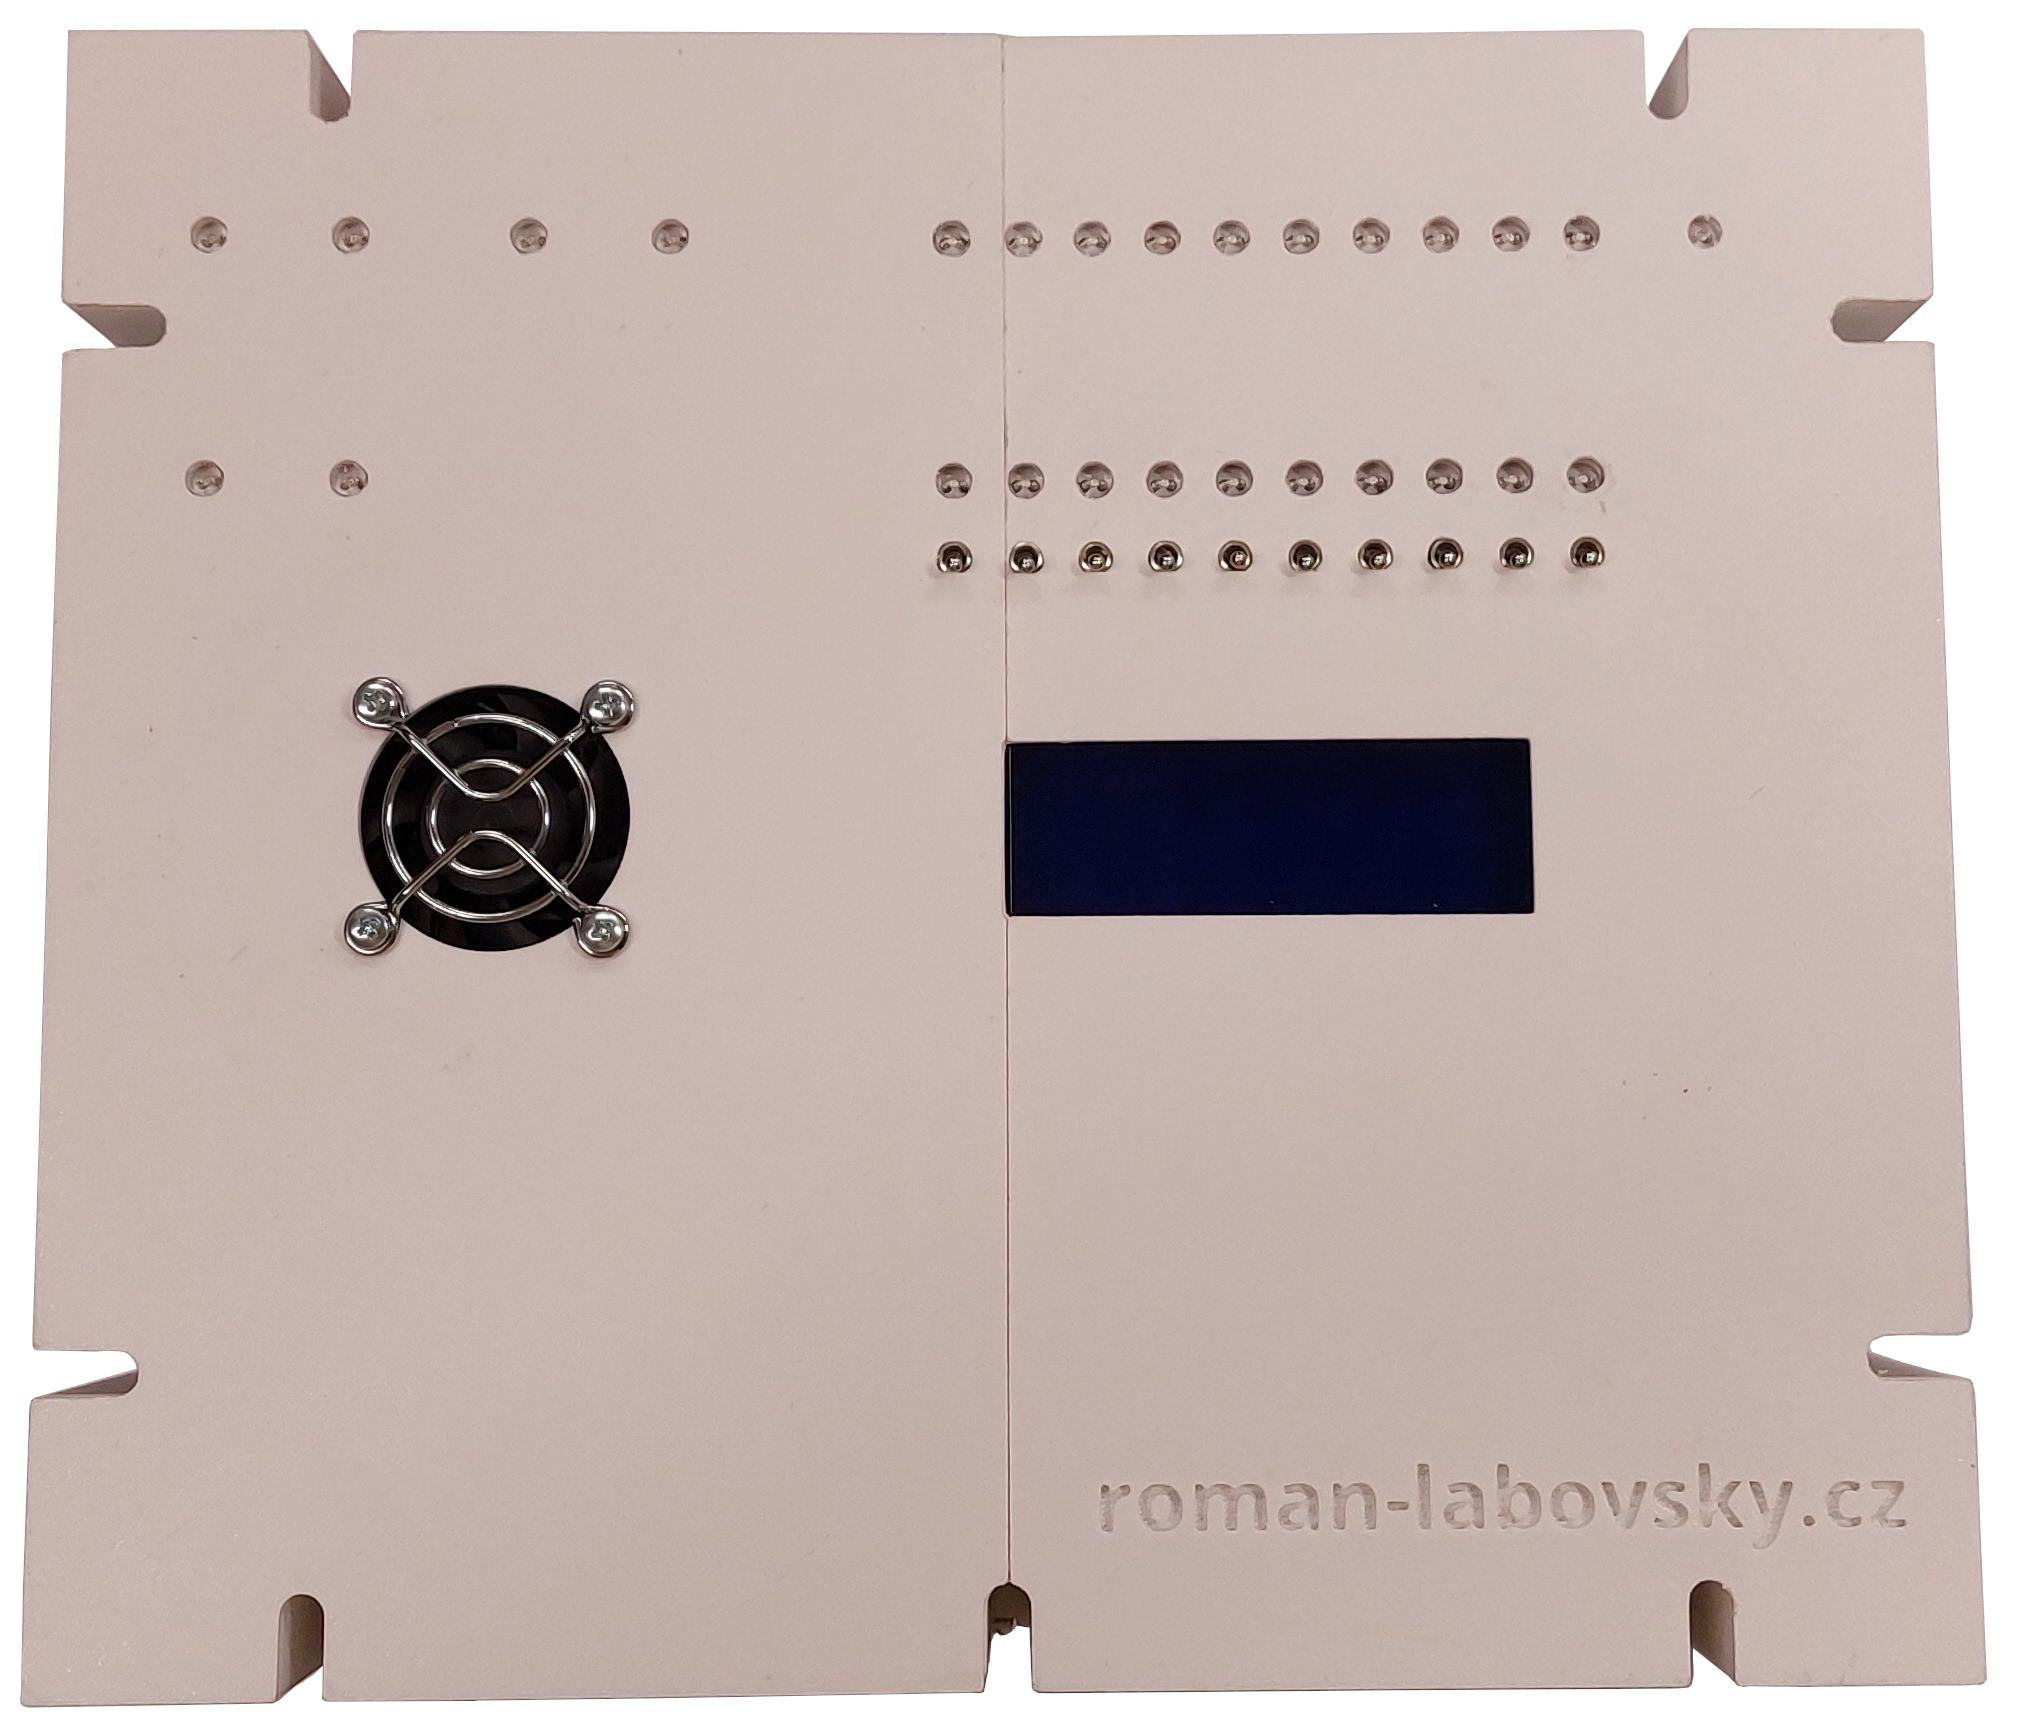
\includegraphics[width=1\textwidth]{pictures/all/hardware/central-control-unit-case-top.jpg}};
      \begin{scope}[x={(image.south east)},y={(image.north west)}]
     	% start SUPPORT GRID
        %\draw[help lines,xstep=.1,ystep=.1] (0,0) grid (1,1);
        %\foreach \x in {0,1,...,9} { \node [anchor=north] at (\x/10,0) {0.\x}; }
        %\foreach \y in {0,1,...,9} { \node [anchor=east] at (0,\y/10) {0.\y}; }
     	% end SUPPORT GRID
                 
          \node[text=red] at (0.1,0.9) {1a};
          \node[text=red] at (0.1,0.76) {1b};
          
          \node[text=red] at (0.17,0.9) {2a};
          \node[text=red] at (0.17,0.76) {2b};
         
          \node[text=red] at (0.26,0.9) {3};
          \node[text=red] at (0.33,0.9) {4};
          
          \node[text=red] at (0.465,0.9) {5a};
          \node[text=red] at (0.505,0.9) {6a};
          \node[text=red] at (0.540,0.9) {7a};
          \node[text=red] at (0.575,0.9) {8a};
          \node[text=red] at (0.610,0.9) {9a};
          \node[text=red] at (0.645,0.9) {10a};
          
          \node[text=red] at (0.465,0.76) {5b};
          \node[text=red] at (0.505,0.76) {6b};
          \node[text=red] at (0.540,0.76) {7b};
          \node[text=red] at (0.575,0.76) {8b};
          \node[text=red] at (0.610,0.76) {9b};
          \node[text=red] at (0.645,0.76) {10b};
          
          \node[text=red] at (0.465,0.64) {5c};
          \node[text=red] at (0.505,0.64) {6c};
          \node[text=red] at (0.540,0.64) {7c};
          \node[text=red] at (0.575,0.64) {8c};
          \node[text=red] at (0.610,0.64) {9c};
          \node[text=red] at (0.645,0.64) {10c};
          
          \node[text=red] at (0.84,0.9) {11};
        \end{scope}
\end{tikzpicture}
\caption{Centrální jednotka s krytem.}
\label{fig:central-control-unit-case-top}
\end{figure}
\end{Czech}

% ========================================

\begin{English}
\subsubsection{Description of Marked Parts}
\end{English}

\begin{Czech}
\subsubsection{Popis označených částí}
\end{Czech}


\begin{English}
\begin{itemize}
  \item \textbf{1a} – Signal LED for 5V (power supply for Raspberry Pi). If blinking, an overcurrent protection is activated.
  \item \textbf{1b} – Signal LED for 3.3V. If lit/blinking, there is a malfunction.
  \item \textbf{2a} – Signal LED for 5V. If blinking, an overcurrent protection is activated.
  \item \textbf{2b} – Signal LED for 3.3V. If lit/blinking, there is a malfunction.
  \item \textbf{3} – Signal LED for 12 V. If lit/blinking, there is a malfunction. Power supply for relay modules.
  \item \textbf{4} – Signal LED for 24V. If lit/blinking, there is a malfunction. Power supply for relay modules.
  \item \textbf{5a} – Signal LED for underfloor heating circulation pump on the ground floor. If lit, the device is turned on.
    \item \textbf{5b} – Signal LED for the underfloor heating circulation pump on the ground floor. If lit, the device is turned on. The switch 5c is turned on.
  \item \textbf{6a} – Signal LED for the underfloor heating circulation pump on the first floor. If lit, the device is turned on.
    \item \textbf{6b} – Signal LED for the underfloor heating circulation pump on the first floor. If lit, the device is turned on. The switch 6c is turned on.
  \item \textbf{7a} – Signal LED for the fireplace circulation pump in the basement. If lit, the device is turned on.
    \item \textbf{7b} – Signal LED for the fireplace circulation pump in the basement. If lit, the device is turned on. The switch 7c is turned on.
  \item \textbf{8a} – Signal LED for the fireplace circulation pump on the ground floor. If lit, the device is turned on.
    \item \textbf{8b} – Signal LED for the fireplace circulation pump on the ground floor. If lit, the device is turned on. The switch 8c is turned on.
  \item \textbf{9a} – Signal LED for the fireplace circulation pump on the first floor. If lit, the device is turned on.
    \item \textbf{9b} – Signal LED for the fireplace circulation pump on the first floor. If lit, the device is turned on. The switch 9c is turned on.
  \item \textbf{10a} – Signal LED for the heating coil. If lit, the device is turned on.
  \item \textbf{10b} – Signal LED for the heating coil. If lit, the device is turned on. The switch 10c is turned on.
    \item \textbf{11} – Signal LED for 5V. If blinking, overcurrent protection is activated. Power supply for signaling the activation/deactivation of corridor thermostats.
\end{itemize}
\end{English}

\begin{Czech}
\begin{itemize}
  \item \textbf{1a} – Signalizační LED pro 5 V (napájení pro Raspberry Pi). Pokud bliká je aktivovaná nadproudová ochrana.
  \item \textbf{1b} – Signalizační LED pro 3,3 V. Pokud svítí/bliká je porucha.
  \item \textbf{2a} – Signalizační LED pro 5 V. Pokud bliká je aktivovaná nadproudová ochrana.
  \item \textbf{2b} – Signalizační LED pro 3,3 V. Pokud svítí/bliká je porucha.
  \item \textbf{3} – Signalizační LED pro 12 V. Pokud svítí/bliká je porucha. Napájení pro relé moduly.
  \item \textbf{4} – Signalizační LED pro 24 V. Pokud svítí/bliká je porucha. Napájení pro relé moduly.
  \item \textbf{5a} – Signalizační LED pro oběhové čerpadlo podlahové vytápění v přízemí. Pokud svítí, zařízení je zapnuto. 
    \item \textbf{5b} – Signalizační LED pro oběhové čerpadlo podlahové vytápění v přízemí. Pokud svítí, zařízení je zapnuto. Je zapnutý přepínač 5c.
  \item \textbf{6a} – Signalizační LED pro oběhové čerpadlo podlahové vytápění v patře. Pokud svítí, zařízení je zapnuto.
    \item \textbf{6b} – Signalizační LED pro oběhové čerpadlo podlahové vytápění v patře. Pokud svítí, zařízení je zapnuto. Je zapnutý přepínač 6c.
  \item \textbf{7a} – Signalizační LED pro oběhové čerpadlo krbu ve sklepě. Pokud svítí, zařízení je zapnuto.
    \item \textbf{7b} – Signalizační LED pro oběhové čerpadlo krbu ve sklepě. Pokud svítí, zařízení je zapnuto. Je zapnutý přepínač 7c.
  \item \textbf{8a} – Signalizační LED pro oběhové čerpadlo krbu v přízemí. Pokud svítí, zařízení je zapnuto.
    \item \textbf{8b} – Signalizační LED pro oběhové čerpadlo krbu v přízemí. Pokud svítí, zařízení je zapnuto. Je zapnutý přepínač 8c.
  \item \textbf{9a} – Signalizační LED pro oběhové čerpadlo krbu v patře. Pokud svítí, zařízení je zapnuto. 
    \item \textbf{9b} – Signalizační LED pro oběhové čerpadlo krbu v patře. Pokud svítí, zařízení je zapnuto. Je zapnutý přepínač 9c.
  \item \textbf{10a} – Signalizační LED pro topnou spirálu. Pokud svítí, zařízení je zapnuto.
  \item \textbf{10b} – Signalizační LED pro topnou spirálu. Pokud svítí, zařízení je zapnuto.  Je zapnutý přepínač 10c. 
    \item \textbf{11} – Signalizační LED pro 5 V. Pokud bliká je aktivovaná nadproudová ochrana. Napájení pro signalizaci sepnutí/vypnutí chodbových termostatů.
\end{itemize}
\end{Czech}


\begin{English}
\tipbox{Note}{Other unmarked switches or outputs are free.}
\end{English}

\begin{Czech}
\tipbox{Poznámka}{Ostatní neoznačené přepínače respektive výstupy jsou volné.}
\end{Czech}


\begin{English}
\begin{figure}[H]
\centering
\begin{tikzpicture}[every text node part/.style={align=center}]
    \node[anchor=south west,inner sep=0] (image) at (0,0)   
   {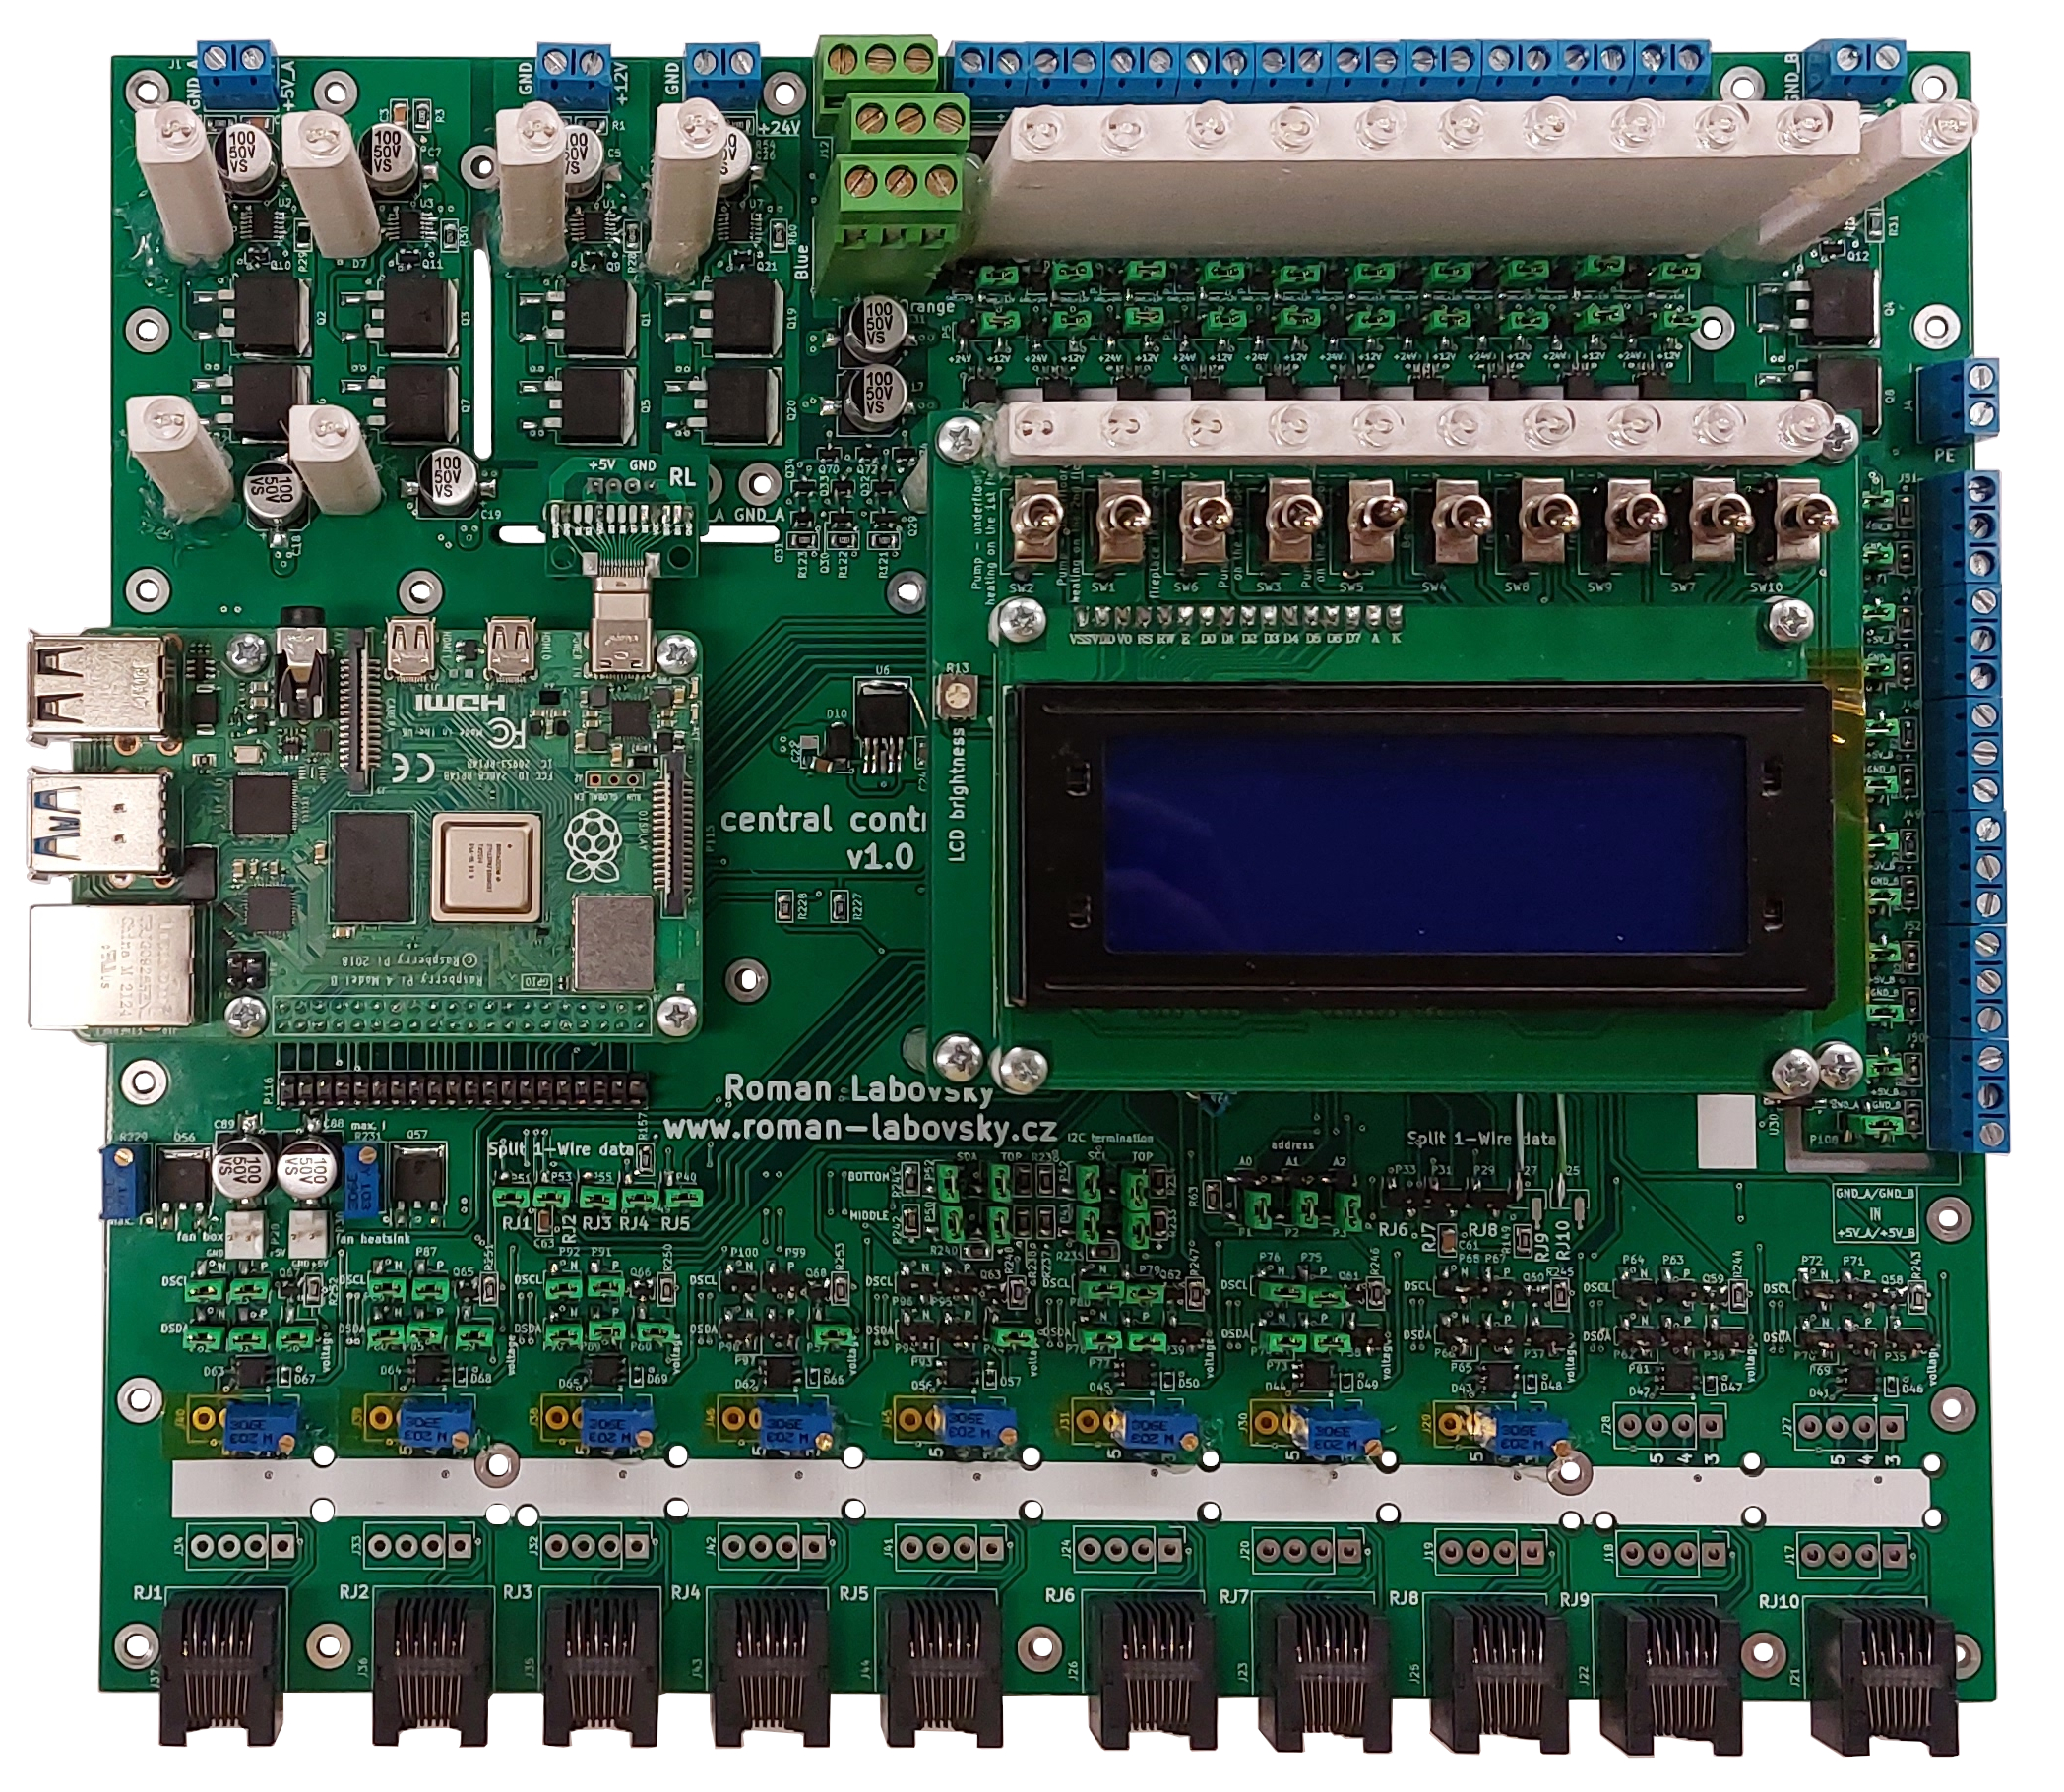
\includegraphics[width=\linewidth]{pictures/all/hardware/central-control-unit-pcb-top.jpg}};
    
     %\node[fill=white,text=orange, draw=orange] at (6.5,12.7) {Sekundární strana Flyback,\\zpětná vazba};
     
    \node[fill=black,text=red, draw=red] at (1.15,4.2) {4}; 
    \draw[red,line width=1mm,rounded corners] (1.5,3.7) rectangle (2.3,4.6);
    
    \node[fill=black,text=green, draw=green] at (3.1,3.95) {5}; 
    \draw[green,line width=1mm,rounded corners] (2.35,3.7) rectangle (2.8,4.2);
    
    \node[fill=black,text=CarnationPink, draw=CarnationPink] at (2.2,5.5) {2}; 
    \draw[CarnationPink,line width=1mm,rounded corners] (0.7,4.6) rectangle (3.5,5.8);
    
    \node[fill=black,text=yellow, draw=yellow] at (5.2,5.2) {3}; 
    \draw[yellow,line width=1mm,rounded corners] (4.2,4.9) rectangle (6.2,5.5);
    \node[fill=black,text=yellow, draw=yellow] at (13.5,5.2) {3}; 
    \draw[yellow,line width=1mm,rounded corners] (12,4.9) rectangle (13.2,5.5);
    
    \node[fill=black,text=orange, draw=orange] at (11.7,13.1) {1};     
    \draw[orange,line width=1mm,rounded corners] (15,12.7) rectangle (8.3,13.5);
    
    \node[fill=white,text=blue, draw=blue] at (16.5,8.5) {8}; 
    \draw[blue,line width=1mm,rounded corners] (16,11.5) rectangle (17,5.5);
    
    \node[fill=black,text=brown, draw=brown] at (1.5,3.2) {6}; 
    \draw[brown,line width=1mm,rounded corners] (1.8,2.9) rectangle (2.8,3.5);
    
    \node[fill=black,text=gray, draw=gray] at (15.5,2.6) {7}; 
    \draw[gray,line width=1mm,rounded corners] (14,0.2) rectangle (17.2,4.7);
    
    \node[fill=black,text=cyan, draw=cyan] at (9.12,5.15) {19};
    \draw[cyan,line width=1mm,rounded corners] (8,4.7) rectangle (10.2,5.6);
        
    \node[fill=black,text=violet, draw=violet] at (11.32,5.85) {20};
    \draw[violet,line width=1mm,rounded corners] (10.8,4.9) rectangle (12,5.5);        
        
    \node[text=white] at (1.9,1) {RJ1};
    \node[text=white] at (3.75,1) {RJ2};
    \node[text=white] at (5.2,1) {RJ3};  
    \node[text=white] at (6.7,1) {RJ4};  
    \node[text=white] at (8.25,1) {RJ5};  
    \node[text=white] at (10.1,1) {RJ6};  
    \node[text=white] at (11.65,1) {RJ7};  
    \node[text=white] at (13.2,1) {RJ8};  
    \node[text=white] at (14.65,1) {RJ9};  
    \node[text=white] at (16.5,1) {RJ10};  
    
    \node[fill=black,text=white, draw=white] at (17.7,11) {9}; 
    \node[fill=black,text=white, draw=white] at (17.8,10) {10};
    \node[fill=black,text=white, draw=white] at (17.85,7.1) {11};
    \node[fill=black,text=white, draw=white] at (17.9,6.1) {12};
    
    \node[fill=black,text=white, draw=white] at (2.1,15.6) {13};
    \node[fill=black,text=white, draw=white] at (5.05,15.6) {14};
    \node[fill=black,text=white, draw=white] at (6.25,15.6) {15};
    \node[fill=black,text=white, draw=white] at (12,15.6) {16};
    \node[fill=black,text=white, draw=white] at (16.2,15.6) {17};
    \node[fill=black,text=white, draw=white] at (17.8,12.2) {18};
    
\end{tikzpicture}
  \caption{The central unit. PCB.}
  \label{fig:central-control-unit-pcb-top}
\end{figure}
\end{English}

\begin{Czech}
\begin{figure}[H]
\centering
\begin{tikzpicture}[every text node part/.style={align=center}]
    \node[anchor=south west,inner sep=0] (image) at (0,0)   
   {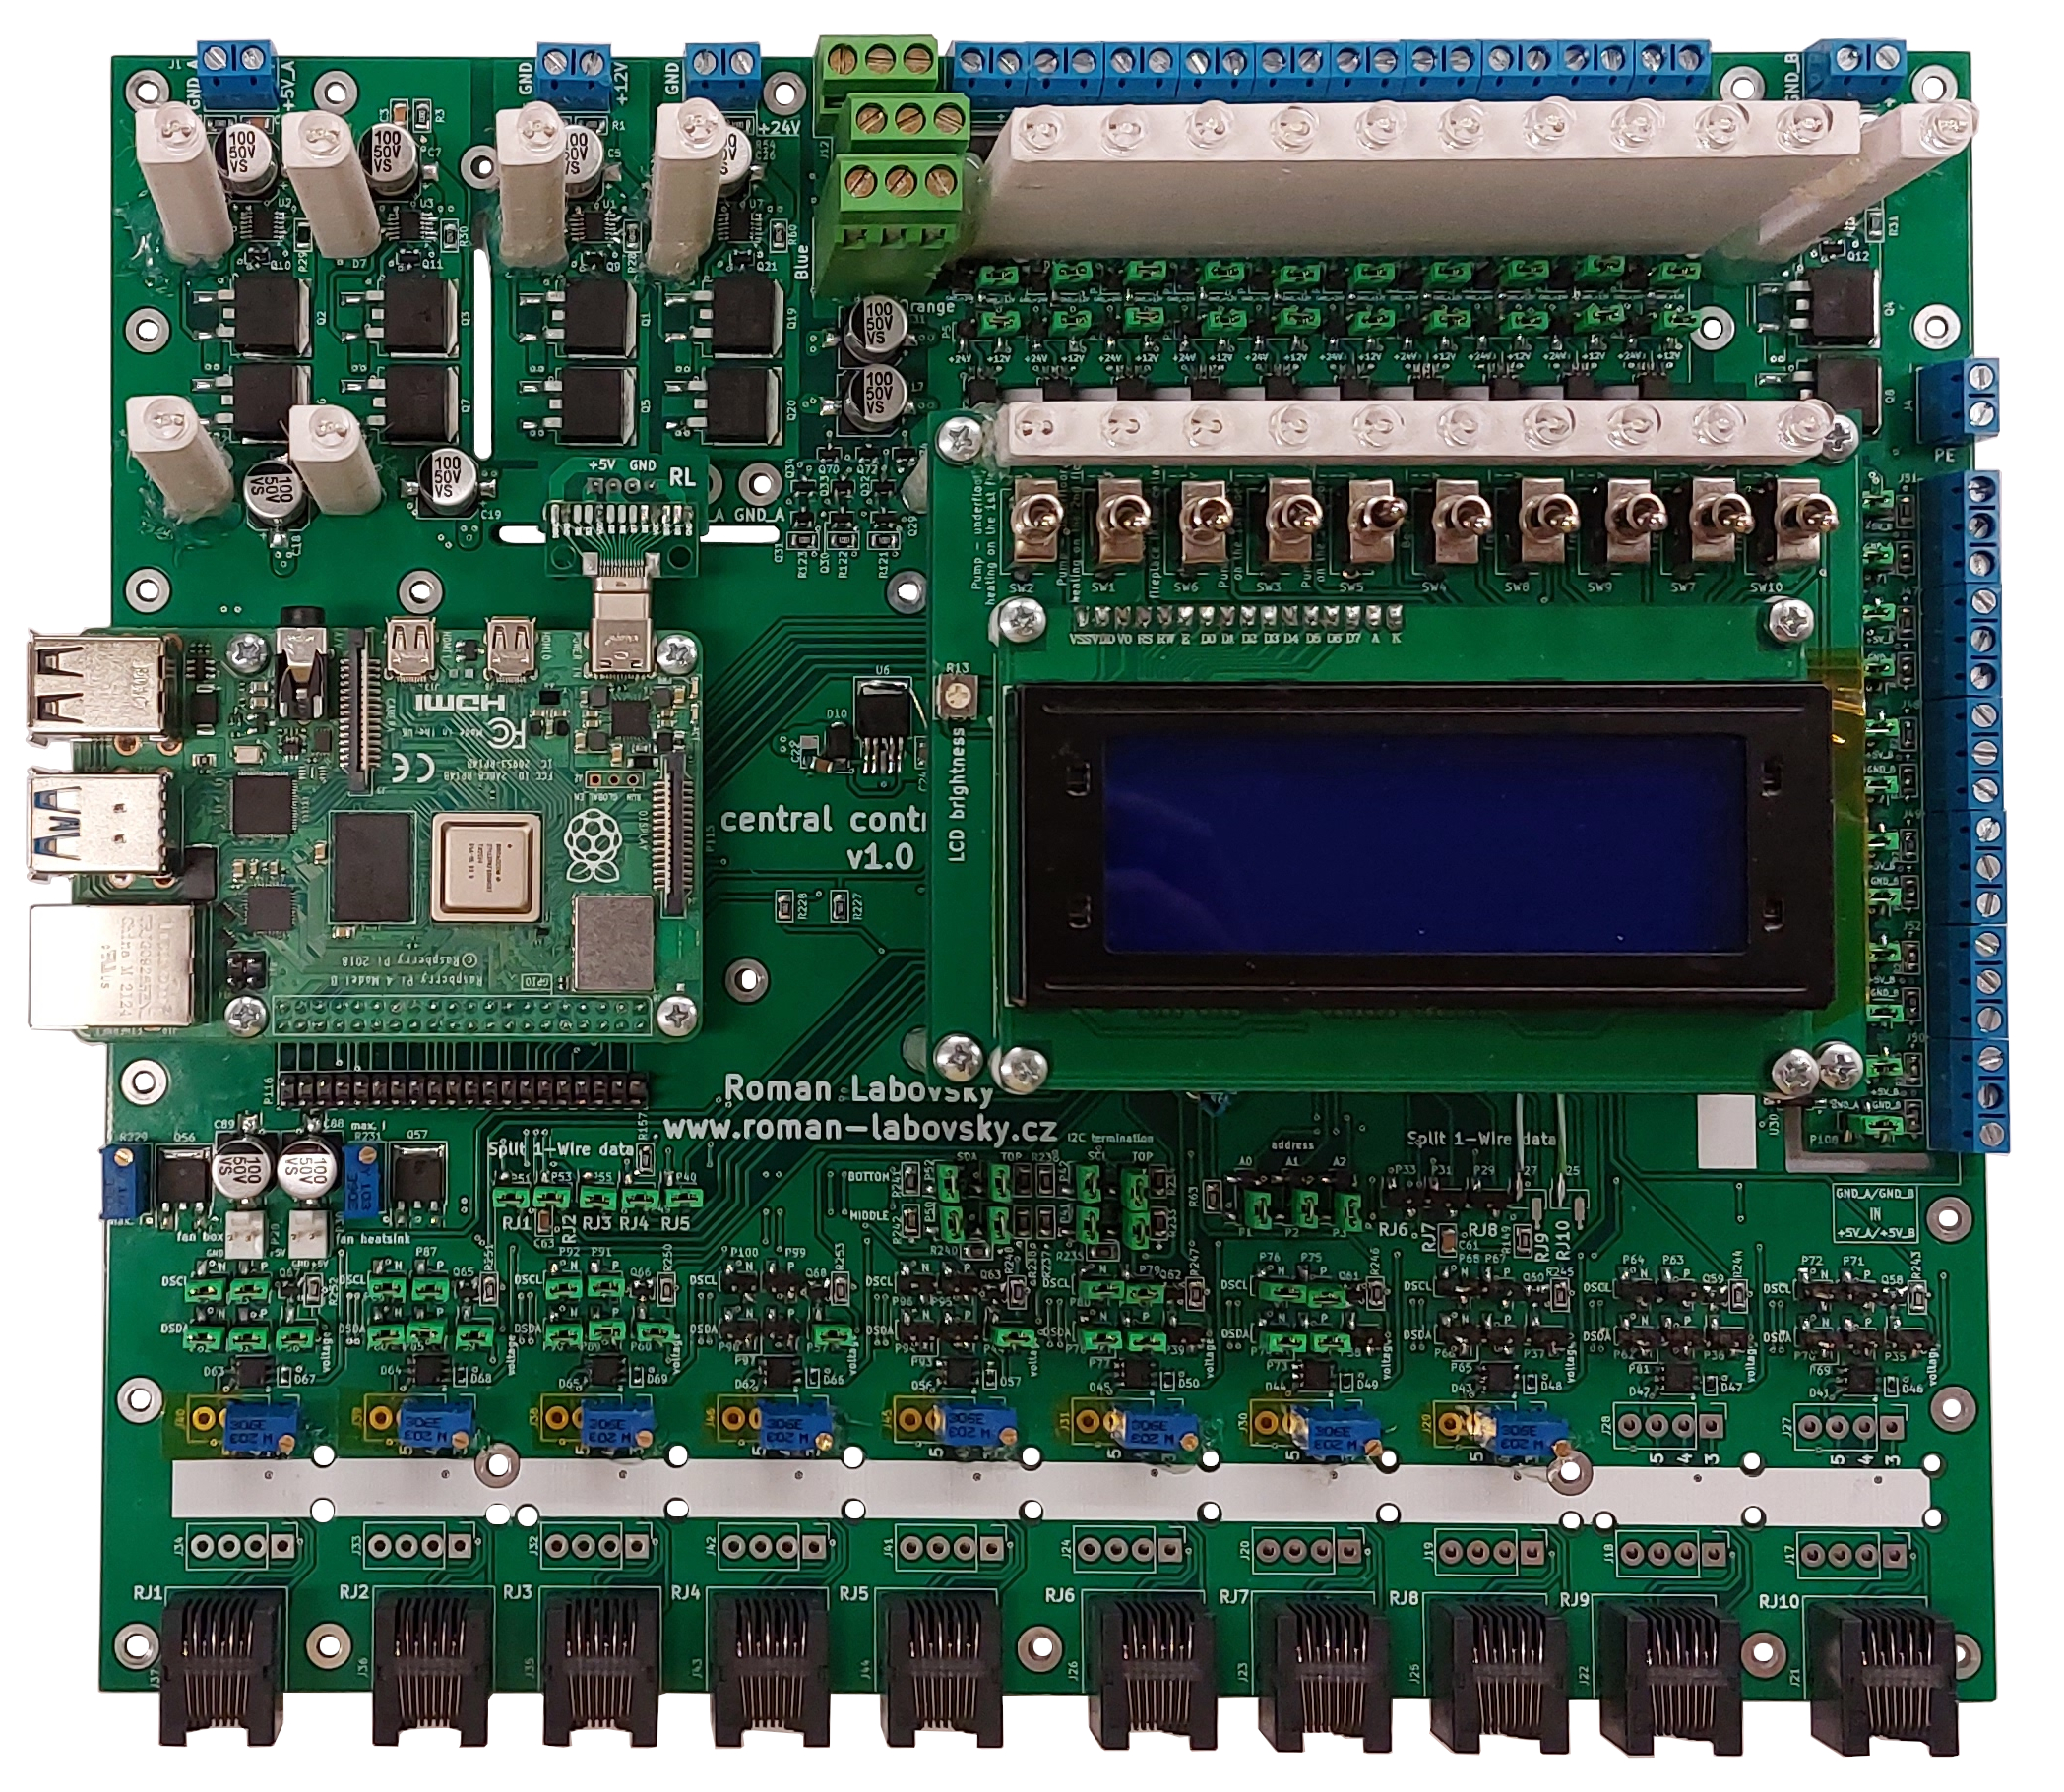
\includegraphics[width=\linewidth]{pictures/all/hardware/central-control-unit-pcb-top.jpg}};
    
     %\node[fill=white,text=orange, draw=orange] at (6.5,12.7) {Sekundární strana Flyback,\\zpětná vazba};
     
    \node[fill=black,text=red, draw=red] at (1.15,4.2) {4}; 
    \draw[red,line width=1mm,rounded corners] (1.5,3.7) rectangle (2.3,4.6);
    
    \node[fill=black,text=green, draw=green] at (3.1,3.95) {5}; 
    \draw[green,line width=1mm,rounded corners] (2.35,3.7) rectangle (2.8,4.2);
    
    \node[fill=black,text=CarnationPink, draw=CarnationPink] at (2.2,5.5) {2}; 
    \draw[CarnationPink,line width=1mm,rounded corners] (0.7,4.6) rectangle (3.5,5.8);
    
    \node[fill=black,text=yellow, draw=yellow] at (5.2,5.2) {3}; 
    \draw[yellow,line width=1mm,rounded corners] (4.2,4.9) rectangle (6.2,5.5);
    \node[fill=black,text=yellow, draw=yellow] at (13.5,5.2) {3}; 
    \draw[yellow,line width=1mm,rounded corners] (12,4.9) rectangle (13.2,5.5);
    
    \node[fill=black,text=orange, draw=orange] at (11.7,13.1) {1};     
    \draw[orange,line width=1mm,rounded corners] (15,12.7) rectangle (8.3,13.5);
    
    \node[fill=white,text=blue, draw=blue] at (16.5,8.5) {8}; 
    \draw[blue,line width=1mm,rounded corners] (16,11.5) rectangle (17,5.5);
    
    \node[fill=black,text=brown, draw=brown] at (1.5,3.2) {6}; 
    \draw[brown,line width=1mm,rounded corners] (1.8,2.9) rectangle (2.8,3.5);
    
    \node[fill=black,text=gray, draw=gray] at (15.5,2.6) {7}; 
    \draw[gray,line width=1mm,rounded corners] (14,0.2) rectangle (17.2,4.7);
    
    \node[fill=black,text=cyan, draw=cyan] at (9.12,5.15) {19};
    \draw[cyan,line width=1mm,rounded corners] (8,4.7) rectangle (10.2,5.6);
        
    \node[fill=black,text=violet, draw=violet] at (11.32,5.85) {20};
    \draw[violet,line width=1mm,rounded corners] (10.8,4.9) rectangle (12,5.5);        
        
    \node[text=white] at (1.9,1) {RJ1};
    \node[text=white] at (3.75,1) {RJ2};
    \node[text=white] at (5.2,1) {RJ3};  
    \node[text=white] at (6.7,1) {RJ4};  
    \node[text=white] at (8.25,1) {RJ5};  
    \node[text=white] at (10.1,1) {RJ6};  
    \node[text=white] at (11.65,1) {RJ7};  
    \node[text=white] at (13.2,1) {RJ8};  
    \node[text=white] at (14.65,1) {RJ9};  
    \node[text=white] at (16.5,1) {RJ10};  
    
    \node[fill=black,text=white, draw=white] at (17.7,11) {9}; 
    \node[fill=black,text=white, draw=white] at (17.8,10) {10};
    \node[fill=black,text=white, draw=white] at (17.85,7.1) {11};
    \node[fill=black,text=white, draw=white] at (17.9,6.1) {12};
    
    \node[fill=black,text=white, draw=white] at (2.1,15.6) {13};
    \node[fill=black,text=white, draw=white] at (5.05,15.6) {14};
    \node[fill=black,text=white, draw=white] at (6.25,15.6) {15};
    \node[fill=black,text=white, draw=white] at (12,15.6) {16};
    \node[fill=black,text=white, draw=white] at (16.2,15.6) {17};
    \node[fill=black,text=white, draw=white] at (17.8,12.2) {18};
    
\end{tikzpicture}
  \caption{Centrální jednotka. DPS.}
  \label{fig:central-control-unit-pcb-top}
\end{figure}
\end{Czech}

% ========================================

\begin{English}
\subsubsection{Description of the Marked Parts}
\end{English}

\begin{Czech}
\subsubsection{Popis označených částí}
\end{Czech}


\begin{English}
\subsubsubsection{The number 1 \colorbox{Orange}{(orange colour)}}
\end{English}

\begin{Czech}
\subsubsubsection{Číslo 1 \colorbox{Orange}{(oranžová barva)}}
\end{Czech}


\begin{English}
There is possible to set +12 V or +24 V for externally connected devices (SSR relays and others) according to the desired voltage range. The selection is made using jumpers, as shown in the figure \ref{fig:pin-header-relays}. For the given output, it is necessary to correctly set both the voltage, either +12V or +24V, and the corresponding ground (GND) for the respective voltage.
\end{English}

\begin{Czech}
Zde je možné nastavit +12 V nebo +24 V pro externí připojené zařízení (SSR relé a jiné) podle požadovaného rozsahu napětí. Volba se dělá pomocí propojek, obrázek \ref{fig:pin-header-relays}. Pro daný výstup je nutné správně nastavit jak napětí tedy +12 V nebo +24 V tak i příslušnou zem (GND) pro dané napětí.
\end{Czech}


\begin{English}
\begin{figure}[H]
    \centering
    \def\svgwidth{0.25\columnwidth}
    \graphicspath{{pictures/all/hardware/svg/}}
    \input{pictures/all/hardware/svg/pin-header-relays.pdf_tex}
    \caption{Selection of voltage for outputs - SSR relays and others. Similar marking is also present on the printed circuit board.}
    \label{fig:pin-header-relays}
\end{figure}
\end{English}

\begin{Czech}
\begin{figure}[H]
    \centering
    \def\svgwidth{0.25\columnwidth}
    \graphicspath{{pictures/all/hardware/svg/}}
    \input{pictures/all/hardware/svg/pin-header-relays.pdf_tex}
    \caption{Výběr napětí pro výstupy - SSR relé a jiné. Podobné značení je i na desce plošných spojů.}
    \label{fig:pin-header-relays}
\end{figure}
\end{Czech}


\begin{English}
\subsubsubsection{The number 2 \colorbox{CarnationPink}{(pink colour)}}
\end{English}

\begin{Czech}
\subsubsubsection{Číslo 2 \colorbox{CarnationPink}{(růžová barva)}}
\end{Czech}


\begin{English}
There is possible to connect external fans to +5V; one connector is already populated for the fan on the central unit cover. Speed regulation is possible with the trimmer next to it.
\end{English}

\begin{Czech}
Zde je možné připojit externí větráky na +5 V, jeden konektor je již osazen pro větrák na krytu centrální jednotky. Regulace otáček je možná příslušný trimry vedle.
\end{Czech}


\begin{English}
\subsubsubsection{The number 3 \colorbox{Yellow}{(yellow colour)}}
\end{English}

\begin{Czech}
\subsubsubsection{Číslo 3 \colorbox{Yellow}{(žlutá barva)}}
\end{Czech}


\begin{English}
To enable the 1-Wire bus (data) on a specific RJ45 connector or UTP, according to RJ45 (numbered RJ1 to RJ10), it is necessary to connect the given jumper in yellow marking. If the 1-Wire bus is not used, remove the jumpers.
\end{English}

\begin{Czech}
Pro povolení 1-Wire sběrnice (data) na daný konektor RJ45 respektive UTP je nutné podle RJ45 (číslo RJ1 až RJ10) propojit daný propoj v žlutém označení. V případě, že nepoužívá sběrnice 1-Wire, propojky odstranit.
\end{Czech}


\begin{English}
\subsubsubsection{The number 4 \colorbox{Red}{(red colour)}}
\end{English}

\begin{Czech}
\subsubsubsection{Číslo 4 \colorbox{Red}{(červená barva)}}
\end{Czech}


\begin{English}
There is differential I$^2$C bus is enabled for the specified RJ45 or UTP using 4 jumpers. If the differential I$^2$C bus is not used, remove the jumpers. Each RJ45 has its own jumpers above the connector.
\end{English}

\begin{Czech}
Zde se pomocí 4 propojek povoluje diferenciální I$^2$C sběrnici pro dané RJ45 respektive UTP. V případě, že nepoužívá sběrnici diferenciální I$^2$C propojky odstranit. Každý RJ45 má své vlastní propojky nad daným konektorem.
\end{Czech}


\begin{English}
\subsubsubsection{The number 5  \colorbox{Green}{(green color)}}
\end{English}

\begin{Czech}
\subsubsubsection{Číslo 5  \colorbox{Green}{(zelená barva)}}
\end{Czech}


\begin{English}
To enable the 1-Wire bus (power) on a specific RJ45 connector or UTP, according to RJ45 (numbered RJ1 to RJ8), it is necessary to connect the given jumper in green marking. If the 1-Wire bus is not used, remove the jumpers. Each RJ45 has its own jumpers above the connector.
\end{English}

\begin{Czech}
Pro povolení 1-Wire sběrnice (napájení) na daný konektor RJ45 respektive UTP je nutné podle RJ45 (číslo RJ1 až RJ8) propojit daný propoj v zeleném označení. V případě, že nepoužívá sběrnice 1-Wire propojky odstranit. Každý RJ45 má své vlastní propojky nad daným konektorem.
\end{Czech}


\begin{English}
\subsubsubsection{The number 6 \colorbox{Brown}{(brown colour)}}
\end{English}

\begin{Czech}
\subsubsubsection{Číslo 6 \colorbox{Brown}{(hněda barva)}}
\end{Czech}


\begin{English}
The pull-up resistor for the 1-Wire bus can be adjusted using trimmers for the RJ45 connector or UTP. Resistance decreases counterclockwise and increases clockwise. Each RJ45 has its own trimmer above the connector.
\end{English}

\begin{Czech}
Pomocí trimrů pro konektor RJ45 respektive UTP lze doladit Pull-up rezistor 1-Wire sběrnice. Proti směru hodinových ručiček se odpor zmenšuje, opačně zvětšuje. Každý RJ45 má svůj vlastní trimer nad daným konektorem.
\end{Czech}


\begin{English}
\subsubsubsection{The number 7 \colorbox{Gray}{(gray colour)}}
\end{English}

\begin{Czech}
\subsubsubsection{Číslo 7 \colorbox{Gray}{(šedá barva)}}
\end{Czech}


\begin{English}
The 1-Wire bus is not available for these two connectors. Only the differential I$^2$C bus is available.
\end{English}

\begin{Czech}
Pro tyto dva konektory není k dispozici 1-Wire sběrnice. Pouze diferenciální I$^2$C sběrnice.
\end{Czech}


\begin{English}
\subsubsubsection{The number 8 \colorbox{Blue}{(blue colour)}}
\end{English}

\begin{Czech}
\subsubsubsection{Číslo 8 \colorbox{Blue}{(modrá barva)}}
\end{Czech}


\begin{English}
There is possible to set +5V\_A or +5V\_B for externally connected devices.
The voltage +5 V\_A is for the same potential external devices as the central unit. The voltage +5 V\_B is galvanically isolated. The selection is made using jumpers, as shown in the figure \ref{fig:pin-header-relays}. It is necessary to have the same jumper for both the voltage and ground.
\end{English}

\begin{Czech}
Zde je možné nastavit +5 V\_A nebo +5 V\_B pro externí připojené zařízení. Napětí +5 V\_A je pro stejný potenciál externího zařízení jako centrální jednotka. Napětí +5 V\_B je galvanicky oddělené. Volba se dělá pomocí propojek, obrázek \ref{fig:pin-header-relays}. Je potřeba mít stejné propojku pro napětí tak i zem.
\end{Czech}


\begin{English}
\begin{figure}[H]
    \centering
    \def\svgwidth{0.25\columnwidth}
    \graphicspath{{pictures/all/hardware/svg/}}
    \input{pictures/all/hardware/svg/pin-header-external-states.pdf_tex}
    \caption{Selection of voltage for outputs - external states. Similar labeling is also present on the printed circuit board.}
    \label{fig:pin-header-external-states}
\end{figure}
\end{English}

\begin{Czech}
\begin{figure}[H]
    \centering
    \def\svgwidth{0.25\columnwidth}
    \graphicspath{{pictures/all/hardware/svg/}}
    \input{pictures/all/hardware/svg/pin-header-external-states.pdf_tex}
    \caption{Výběr napětí pro výstupy - externí stavy. Podobné značení je i na desce plošných spojů.}
    \label{fig:pin-header-external-states}
\end{figure}
\end{Czech}


\begin{English}
\subsubsubsection{The number 9, 10}
\end{English}

\begin{Czech}
\subsubsubsection{Číslo 9, 10}
\end{Czech}


\begin{English}
The middle pin of connector 9 or 10 is connected to the corridor thermostat from the ground floor respectively from the first floor. Voltage +5V\_B is used for the middle pin. The connection of the device to the connector is shown in the figure \ref{fig:terminal-block-external-state}. Similar marking is also present on the printed circuit board. It is necessary to have a jumper for both the voltage +5 V\_B and GND\_B.
\end{English}

\begin{Czech}
Na prostřední pin konektoru 9 respektive 10 je připojen chodbový termostat z přízemí respektive z patra. Využívá se +5 V\_B a prostřední pin. Zapojení zařízení do konektoru je na obrázku \ref{fig:terminal-block-external-state}. Obdobné značení je i na desce plošných spojů. Je potřeba mít propojku na napětí +5 V\_B a  GND\_B.
\end{Czech}


\begin{English}
\subsubsubsection{The number 11, 12}
\end{English}

\begin{Czech}
\subsubsubsection{Číslo 11, 12}
\end{Czech}


\begin{English}
The middle pin of connector 11 or 12 is connected to the external state for controlling the circulation pump from the zone controller on the ground floor respectively from the first floor. The middle pin of the connector is used.
The connection of the device to the connector is shown in the figure \ref{fig:terminal-block-external-state}. Similar marking is also present on the printed circuit board. The orientation of the connector is in the figure \ref{fig:terminal-block-external-state} is identical to the orientation in the figure \ref{fig:central-control-unit-pcb-top}. It is necessary to have a jumper for both the voltage +5V\_A and GND\_A.
\end{English}

\begin{Czech}
Na prostřední pin konektoru 11 respektive 12 je připojen externí stav pro ovládání oběhového podlahového čerpadla ze zónového regulátoru v přízemí respektive z patra. Využívá se prostřední pin daného konektoru. Zapojení zařízení do konektoru je na obrázku \ref{fig:terminal-block-external-state}. Obdobné značení je i na desce plošných spojů. Orientace konektoru na obrázku \ref{fig:terminal-block-external-state} je shodná s orientací na \ref{fig:central-control-unit-pcb-top}. Je potřeba mít propojku na napětí +5 V\_A a  GND\_A.
\end{Czech}


\begin{English}
\begin{figure}[H]
    \centering
    \def\svgwidth{0.15\columnwidth}
    \graphicspath{{pictures/all/hardware/svg/}}
    \input{pictures/all/hardware/svg/terminal-block-external-states.pdf_tex}
    \caption{The connection of the external device to the terminal block for external states. Similar marking is also present on the printed circuit board.}
    \label{fig:terminal-block-external-state}
\end{figure}
\end{English}

\begin{Czech}
\begin{figure}[H]
    \centering
    \def\svgwidth{0.15\columnwidth}
    \graphicspath{{pictures/all/hardware/svg/}}
    \input{pictures/all/hardware/svg/terminal-block-external-states.pdf_tex}
    \caption{Zapojení externího zařízení na svorkovnici pro externí stavy. Obdobné značení je i na desce plošných spojů.}
    \label{fig:terminal-block-external-state}
\end{figure}
\end{Czech}


\begin{English}
\subsubsubsection{Connectors from RJ1 to RJ10}
\end{English}

\begin{Czech}
\subsubsubsection{Konektory RJ1 až RJ10}
\end{Czech}


\begin{English}
Connectors from RJ1 to RJ10 are used for connecting devices utilizing either the 1-Wire bus or the differential I$^2$C bus.
\end{English}

\begin{Czech}
Konektory RJ1 až RJ10 slouží pro připojení zařízení využívající 1-Wire sběrnici nebo diferenciální I$^2$C sběrnici.
\end{Czech}


\begin{English}
\begin{itemize}
  \item RJ1 – the cellar fireplace, connection of 1-Wire bus for a thermocouple, differential I$^2$C bus for a display.
  \item RJ2 – the ground floor fireplace, connection of 1-Wire bus for a thermocouple, differential I$^2$C bus for a display.
  \item RJ3 – the first floor fireplace, connection of 1-Wire bus for thermocouple, differential I$^2$C bus for a display.
  \item RJ4 – the hot water tank on the first floor, connection of 1-Wire bus for temperature sensors.
  \item RJ5 – the outdoor temperature sensor, connection of 1-Wire bus.
  \item RJ6 – the distribution box on the ground floor, connection of differential I$^2$C bus for controlling valves.
  \item RJ7 – the distribution box on the first floor, connection of differential I$^2$C bus for controlling valves.
\end{itemize}
\end{English}

\begin{Czech}
\begin{itemize}
  \item RJ1 – krb sklep, připojení 1-Wire sběrnice pro termočlánek, diferenciální I$^2$C sběrnice pro displej.
  \item RJ2 – krb přízemí, připojení 1-Wire sběrnice pro termočlánek, diferenciální I$^2$C sběrnice pro displej.
  \item RJ3 – krb patro, připojení 1-Wire sběrnice pro termočlánek, diferenciální I$^2$C sběrnice pro displej.
  \item RJ4 – zásobník otopné vody patro, připojení 1-Wire sběrnice pro teplotní senzory.
  \item RJ5 – venkovní teplotní senzor, připojení 1-Wire sběrnice.
  \item RJ6 – rozdělovač v přízemí, připojení diferenciální I$^2$C sběrnice pro ovládání ventilů.
  \item RJ7 – rozdělovač v patře, připojení diferenciální I$^2$C sběrnice pro ovládání ventilů.
\end{itemize}
\end{Czech}


\begin{English}
\tipbox{Note}{The other RJ45 connectors (RJ8, RJ9, RJ10) are available. RJ9 and RJ10 connectors support only the differential I$^2$C bus.}
\end{English}

\begin{Czech}
\tipbox{Poznámka}{Ostatní konektory RJ45 (RJ8, RJ9, RJ10) jsou volné. Konektory RJ9, RJ10 podporují pouze diferenciální I$^2$C sběrnici.}
\end{Czech}


\newpage
\begin{English}
\subsubsubsection{The number 13, 14, 15, 17}
\end{English}

\begin{Czech}
\subsubsubsection{Číslo 13, 14, 15, 17}
\end{Czech}


\begin{English}
Connectors for connection of +5V, +12V, +24V, +5V. The maximum allowed voltage is written on the PCB.
The power supply connection to the connector is shown in the figure \ref{fig:central-control-unit-terminal-blocks-power-supply}. Orientation of the connector in the figure \ref{fig:central-control-unit-terminal-blocks-power-supply} is the same as the orientation in figure  \ref{fig:central-control-unit-pcb-top}.
\end{English}

\begin{Czech}
Konektory pro připojení +5 V, +12 V, +24 V, +5 V. Maximální dovolené napětí je napsáno na DPS. Zapojení napájení do konektoru je na obrázku \ref{fig:central-control-unit-terminal-blocks-power-supply}. Orientace konektoru na obrázku \ref{fig:central-control-unit-terminal-blocks-power-supply} je shodná s orientací na \ref{fig:central-control-unit-pcb-top}.
\end{Czech}


\begin{English}
\begin{figure}[H]
    \centering
    \def\svgwidth{0.15\columnwidth}
    \graphicspath{{pictures/all/hardware/svg/}}
    \input{pictures/all/hardware/svg/central-control-unit-terminal-blocks-power-supply.pdf_tex}
    \caption{Connector for power supply voltages. The maximum allowed voltage is written on the PCB. Similar marking is also present on the printed circuit board.}
    \label{fig:central-control-unit-terminal-blocks-power-supply}
\end{figure}
\end{English}

\begin{Czech}
\begin{figure}[H]
    \centering
    \def\svgwidth{0.15\columnwidth}
    \graphicspath{{pictures/all/hardware/svg/}}
    \input{pictures/all/hardware/svg/central-control-unit-terminal-blocks-power-supply.pdf_tex}
    \caption{Konektor pro připojení napájecích napětí. Maximální dovolené napětí je napsáno na DPS. Obdobné značení je i na desce plošných spojů.}
    \label{fig:central-control-unit-terminal-blocks-power-supply}
\end{figure}
\end{Czech}


\begin{English}
\tipbox{Attention}{The maximum allowed voltage is written on the PCB.}
\end{English}

\begin{Czech}
\tipbox{Pozor}{Maximální dovolené napětí je napsáno na DPS.}
\end{Czech}


\begin{English}
\subsubsubsection{The number 16}
\end{English}

\begin{Czech}
\subsubsubsection{Číslo 16}
\end{Czech}


\begin{English}
Connectors for connecting external devices (SSR relays and others). The connection of devices to the connector is shown in the figure \ref{fig:central-control-unit-terminal-block-relays}. Similar marking is also present on the printed circuit board. The orientation of the connector in the figure \ref{fig:central-control-unit-terminal-block-relays} is the same as the orientation in \ref{fig:central-control-unit-pcb-top}.
\end{English}

\begin{Czech}
Konektory pro připojení externích zařízení (SSR relé a jiné).  Zapojení zařízení do konektoru je na obrázku \ref{fig:central-control-unit-terminal-block-relays}. Obdobné značení je i na desce plošných spojů. Orientace konektoru na obrázku \ref{fig:central-control-unit-terminal-block-relays} je shodná s orientací na \ref{fig:central-control-unit-pcb-top}.
\end{Czech}


\begin{English}
\begin{figure}[H]
    \centering
    \def\svgwidth{0.15\columnwidth}
    \graphicspath{{pictures/all/hardware/svg/}}
    \input{pictures/all/hardware/svg/central-control-unit-terminal-block-relays.pdf_tex}
    \caption{Connector for connecting external devices (SSR relays and others). Similar marking is also present on the printed circuit board.}
    \label{fig:central-control-unit-terminal-block-relays}
\end{figure}
\end{English}

\begin{Czech}
\begin{figure}[H]
    \centering
    \def\svgwidth{0.15\columnwidth}
    \graphicspath{{pictures/all/hardware/svg/}}
    \input{pictures/all/hardware/svg/central-control-unit-terminal-block-relays.pdf_tex}
    \caption{Konektor pro připojení externích zařízení (SSR relé a jiné). Obdobné značení je i na desce plošných spojů.}
    \label{fig:central-control-unit-terminal-block-relays}
\end{figure}
\end{Czech}


\begin{English}
\subsubsubsection{The number 18}
\end{English}

\begin{Czech}
\subsubsubsection{Číslo 18}
\end{Czech}


\begin{English}
Connector for connecting the protective earth wire (PE). Both terminals can be connected to the PE wire.
\end{English}

\begin{Czech}
Konektor pro připojení ochranného vodiče PE. Obě svorky lze připojit na vodič PE.
\end{Czech}


\begin{English}
\subsubsubsection{The number 19 \colorbox{Cyan}{cyan colour}}
\end{English}

\begin{Czech}
\subsubsubsection{Číslo 19 \colorbox{Cyan}{tyrkysová barva}}
\end{Czech}


\begin{English}
Enabling the I$^2$C bus on RJ45 connectors. Jumpers connect terminating resistors between wires. Leave all connected.
\end{English}

\begin{Czech}
Povolení I$^2$C sběrnice na konektory RJ45. Propojky připojují ukončovací rezistory mezi vodiče. Nechat všechny zapojené.
\end{Czech}


\begin{English}
\subsubsubsection{The number 20 \colorbox{Violet}{violet colour}}
\end{English}

\begin{Czech}
\subsubsubsection{Číslo 20 \colorbox{Violet}{fialová barva}}
\end{Czech}


\begin{English}
The jumpers set the address for the SPI device (reset circuit for the 1-Wire bus power). No need to reconfigure.
\end{English}

\begin{Czech}
Propojky nastavují adresu pro SPI obvod (obvod pro reset napájení 1-Wire sběrnice).  Netřeba přenastavovat.
\end{Czech}

% ====================  STOP Central Control Unit ====================

% ====================  START Zone Controller ====================

\newpage
\begin{English}
\subsection{The Zone Controller}
\end{English}

\begin{Czech}
\subsection{Zónový regulátor}
\end{Czech}


\begin{English}
In the figure \ref{fig:zone-controller-panel-top}, there is the zone controller with a description of individual LEDs and switches.
\end{English}

\begin{Czech}
Na obrázku \ref{fig:zone-controller-panel-top} je zónový regulátor s popisem jednotlivých LED a přepínačů.
\end{Czech}


\begin{English}
\begin{figure}[H]
\centering
\begin{tikzpicture}[font=\sffamily]
     \node[anchor=south west,inner sep=0] (image) at (0,0) {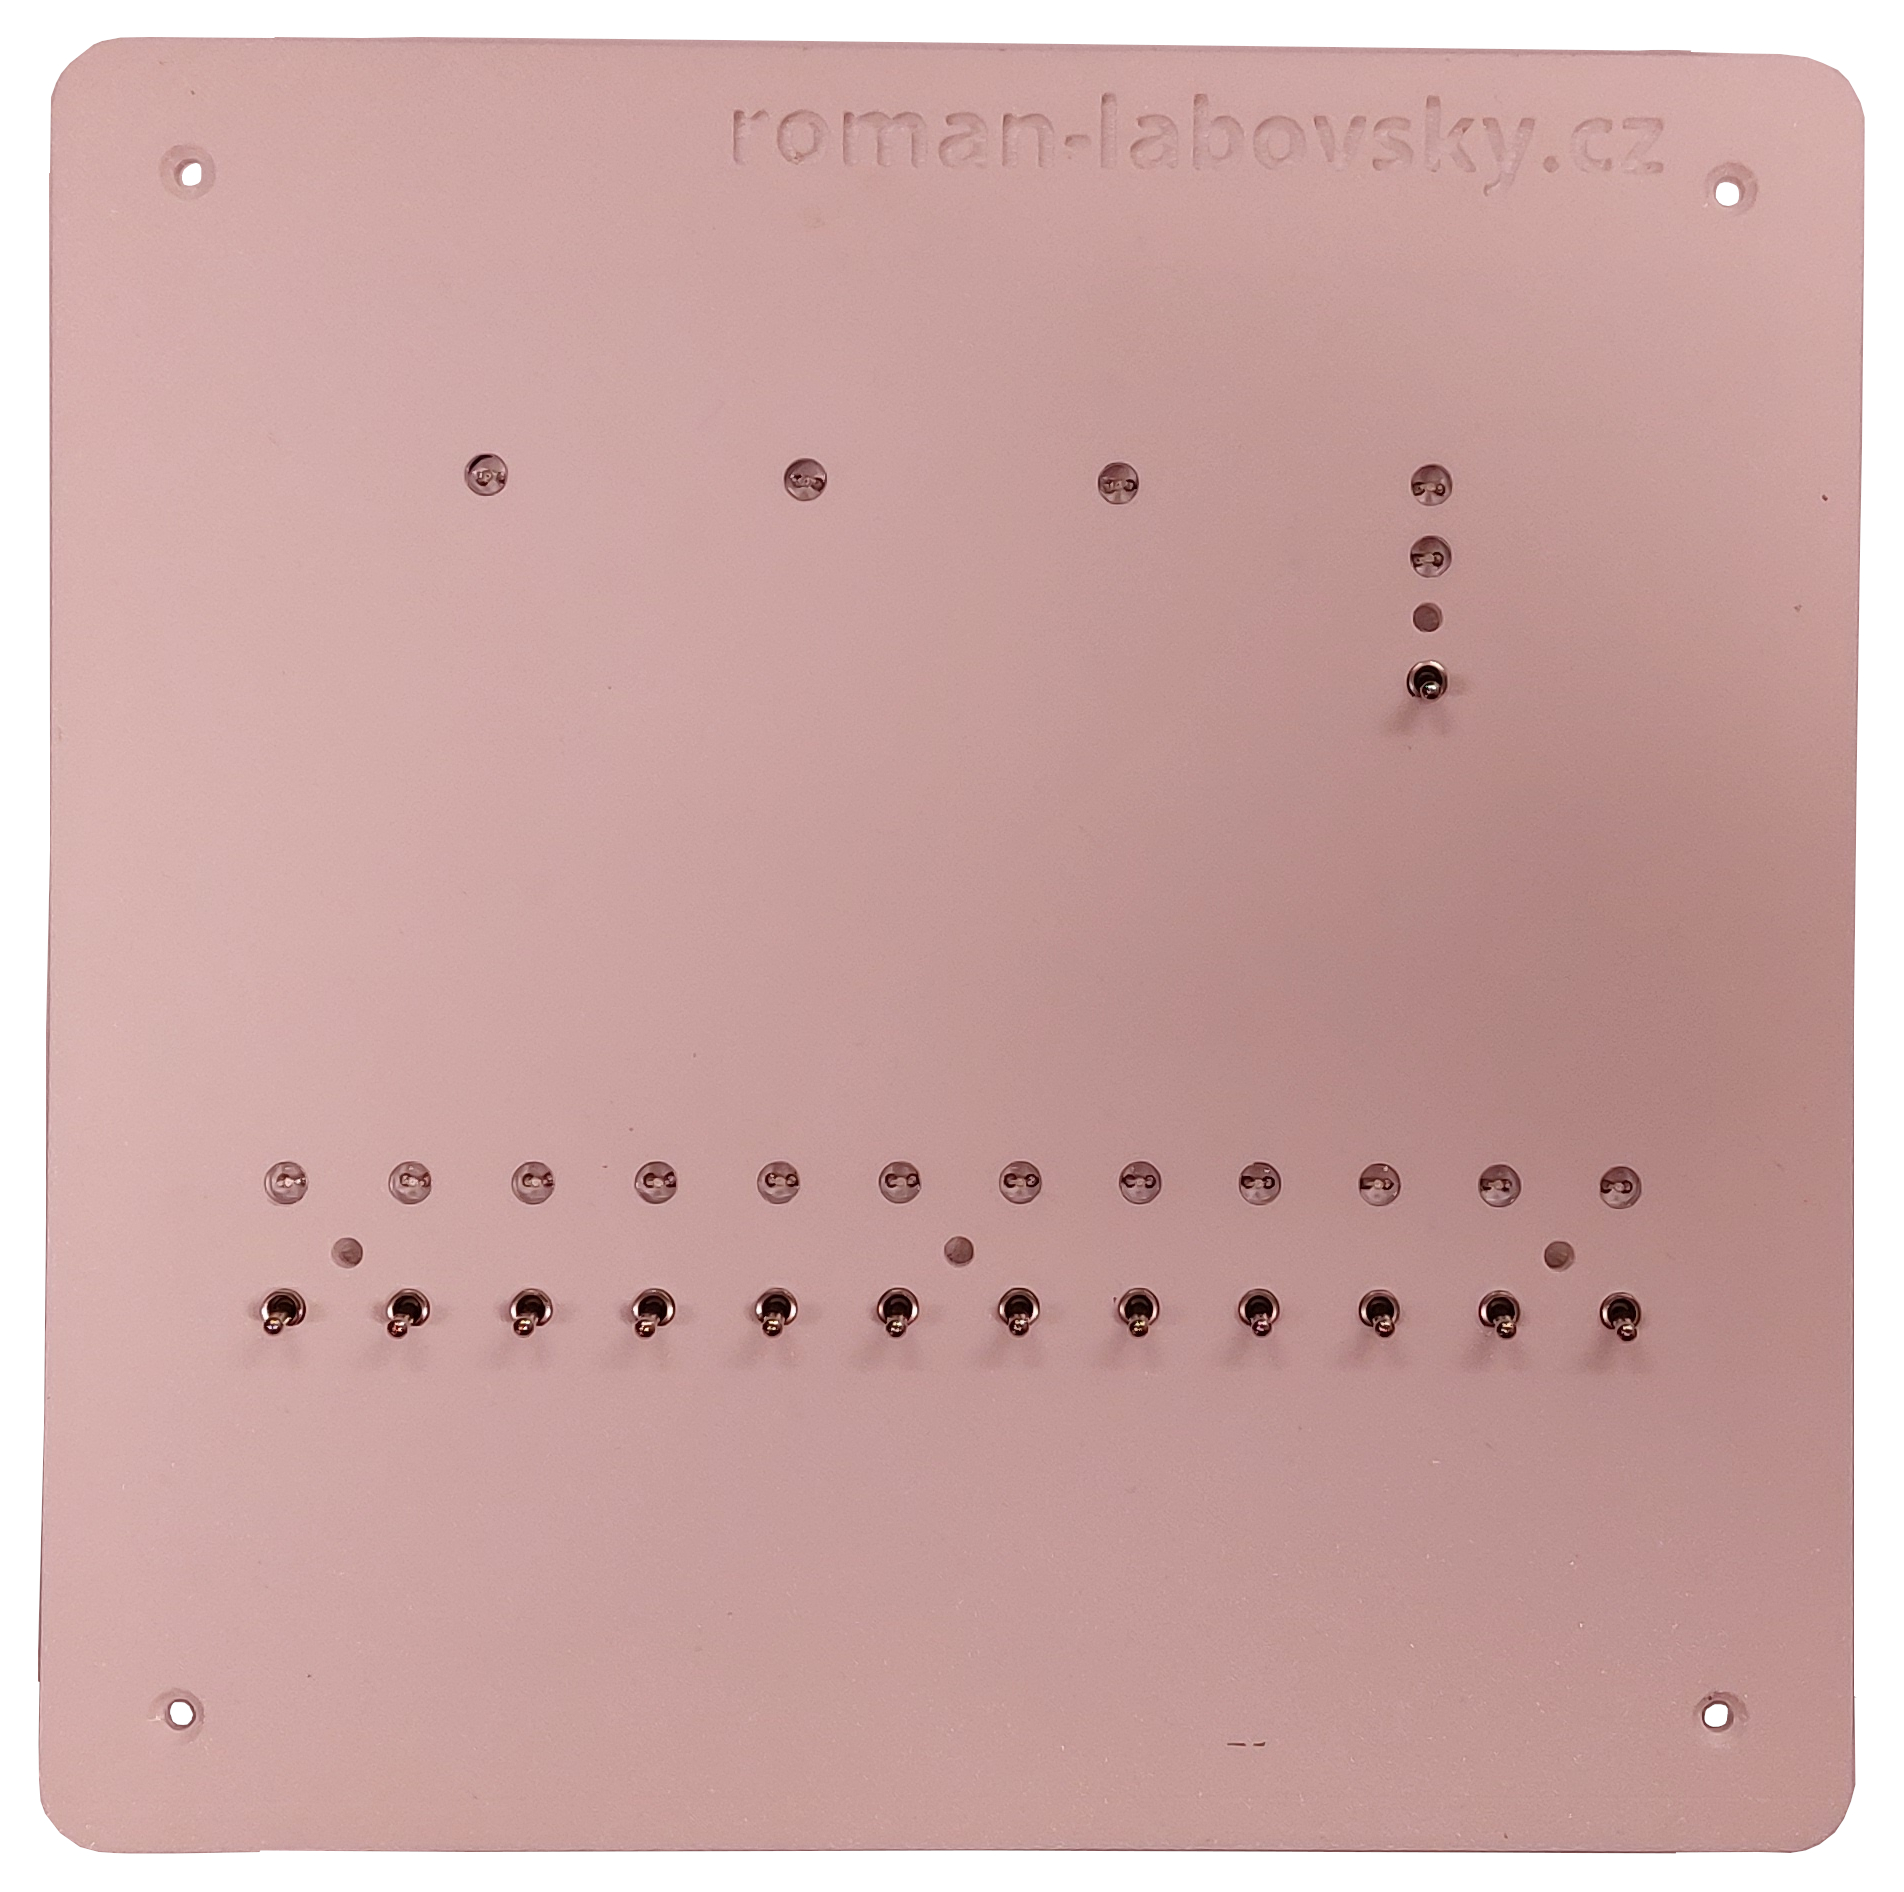
\includegraphics[width=1\textwidth]{pictures/all/hardware/zone-controller-panel-top.jpg}};
      \begin{scope}[x={(image.south east)},y={(image.north west)}]
     	% start SUPPORT GRID
        %\draw[help lines,xstep=.1,ystep=.1] (0,0) grid (1,1);
        %\foreach \x in {0,1,...,9} { \node [anchor=north] at (\x/10,0) {0.\x}; }
        %\foreach \y in {0,1,...,9} { \node [anchor=east] at (0,\y/10) {0.\y}; }
     	% end SUPPORT GRID
                 
          \node[text=red] at (0.255,0.78) {1};        
          \node[text=red] at (0.425,0.78) {2};
          \node[text=red] at (0.585,0.78) {3};        
          \node[text=red] at (0.755,0.78) {4a};
          \node[text=red] at (0.78,0.705) {4b};
          \node[text=red] at (0.78,0.64) {4c};    
          \node[text=red] at (0.505,0.4) {5};    
                  
        \end{scope}
\end{tikzpicture}
\caption{The zone regulator with a cover.}
\label{fig:zone-controller-panel-top}
\end{figure}
\end{English}

\begin{Czech}
\begin{figure}[H]
\centering
\begin{tikzpicture}[font=\sffamily]
     \node[anchor=south west,inner sep=0] (image) at (0,0) {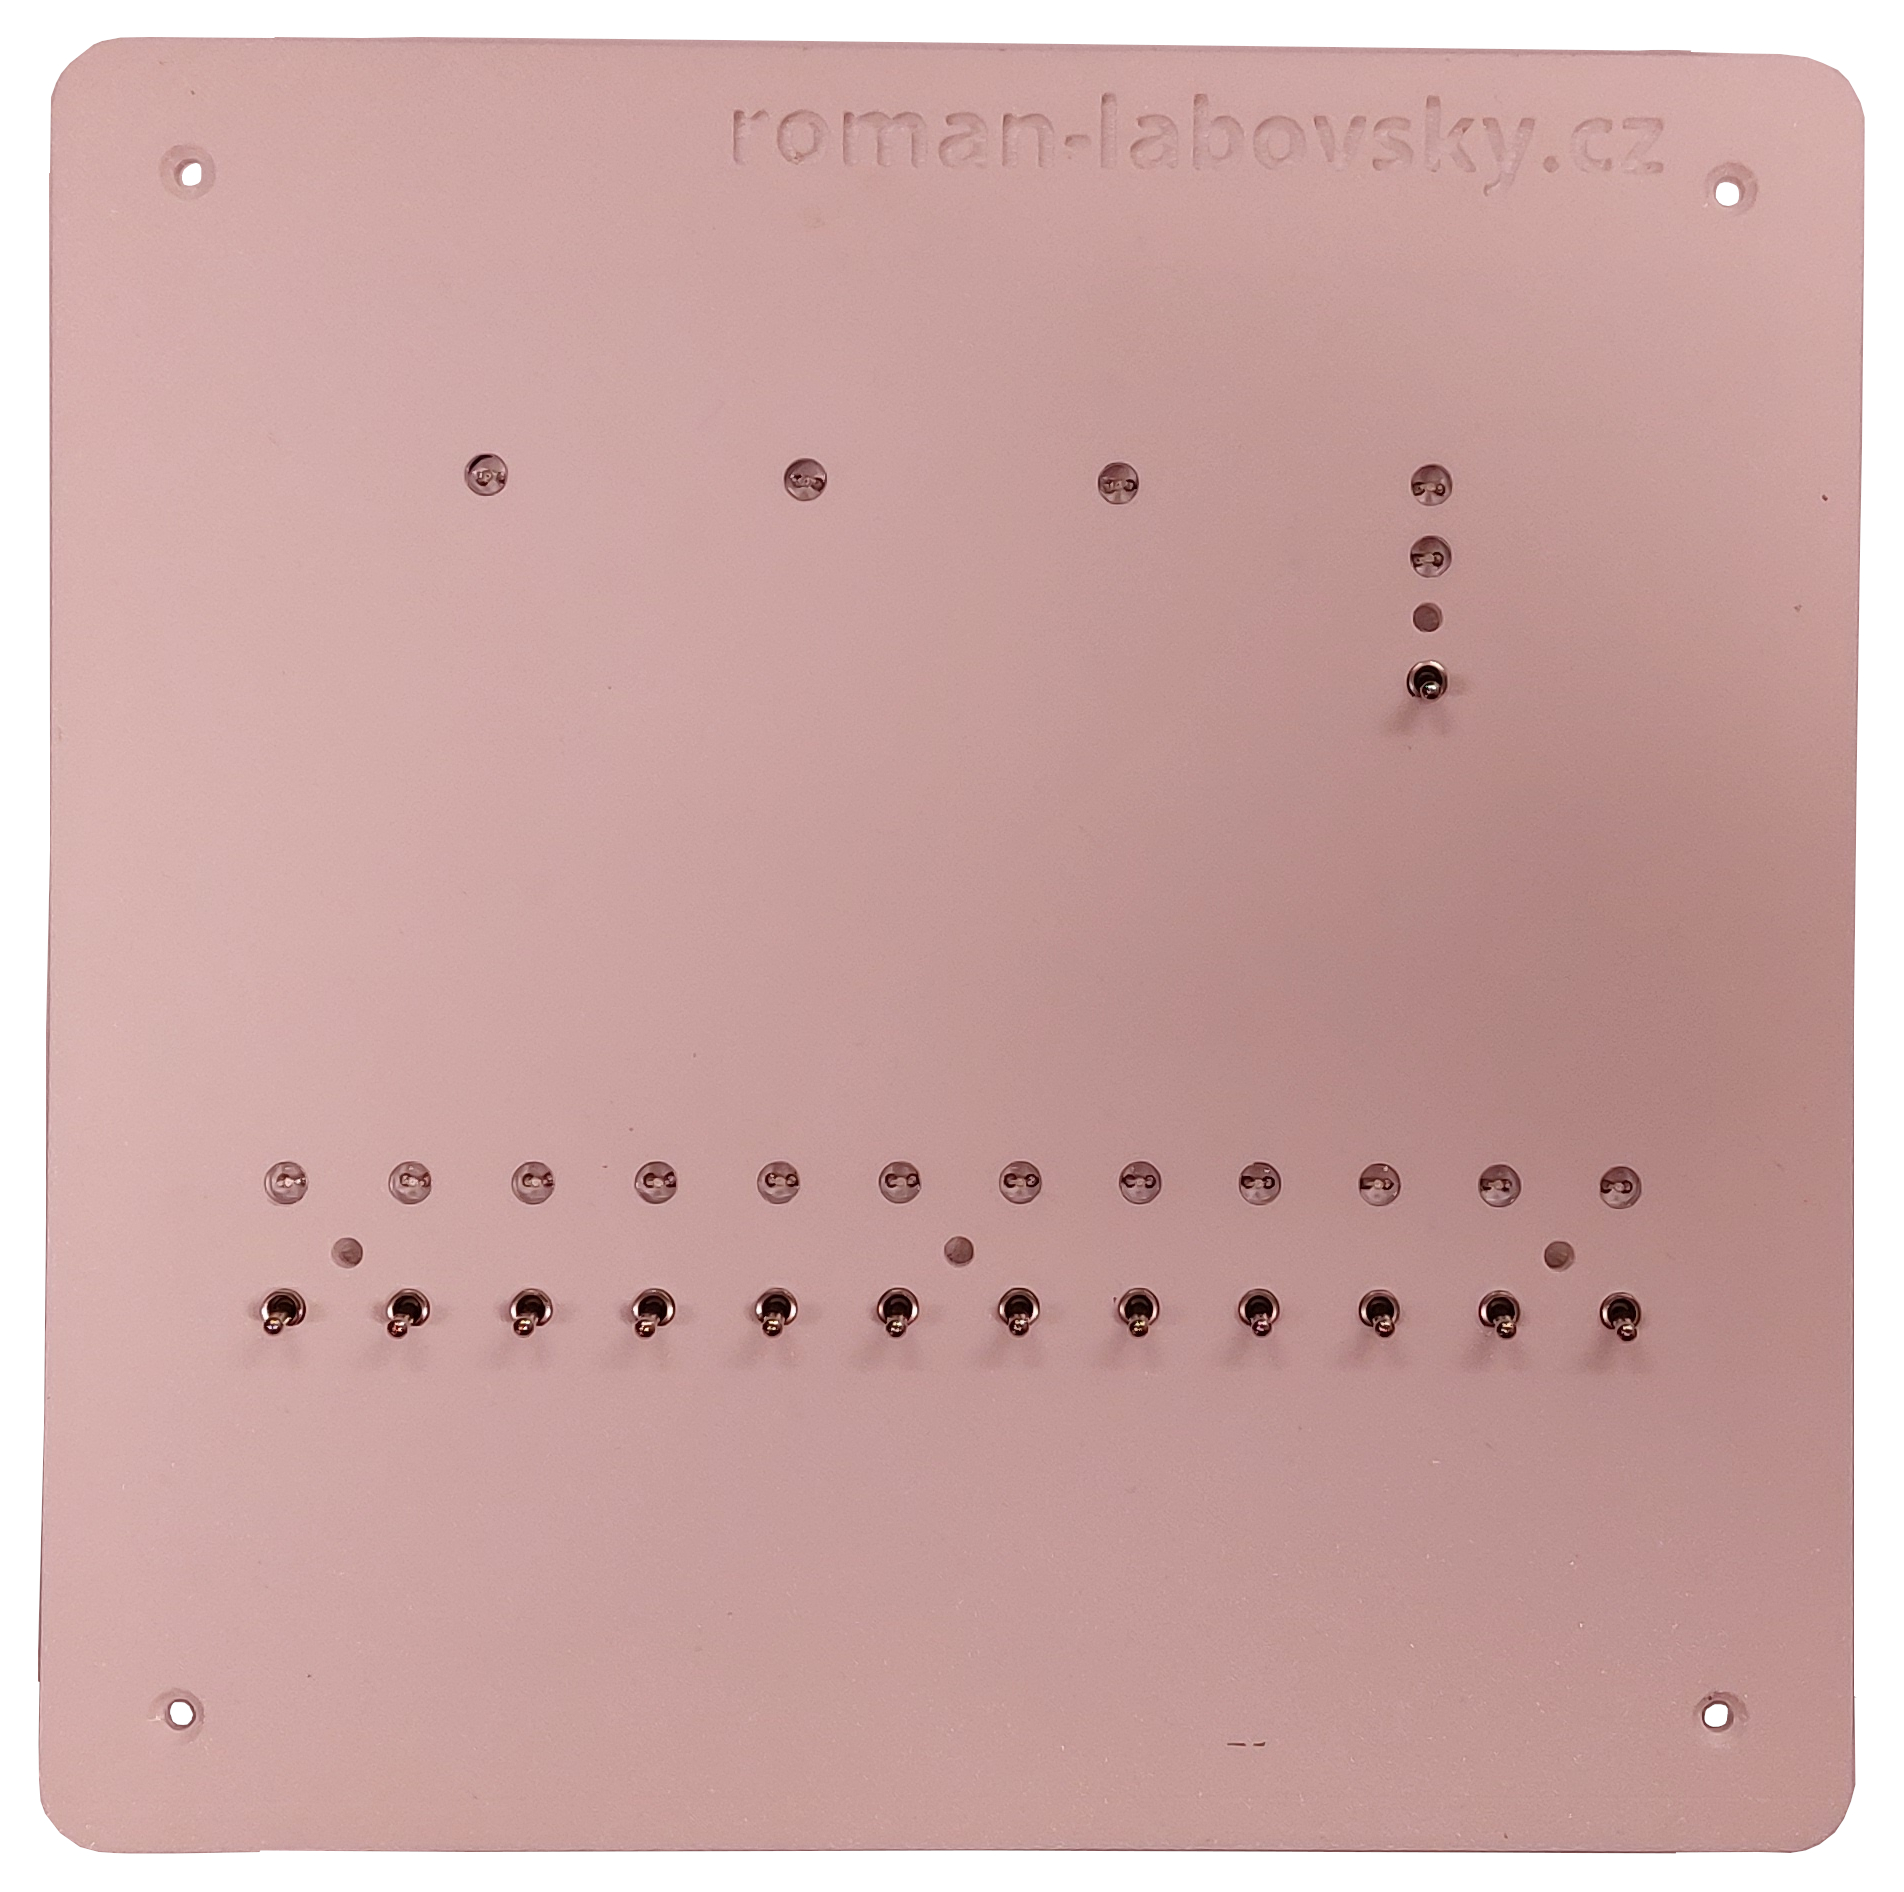
\includegraphics[width=1\textwidth]{pictures/all/hardware/zone-controller-panel-top.jpg}};
      \begin{scope}[x={(image.south east)},y={(image.north west)}]
     	% start SUPPORT GRID
        %\draw[help lines,xstep=.1,ystep=.1] (0,0) grid (1,1);
        %\foreach \x in {0,1,...,9} { \node [anchor=north] at (\x/10,0) {0.\x}; }
        %\foreach \y in {0,1,...,9} { \node [anchor=east] at (0,\y/10) {0.\y}; }
     	% end SUPPORT GRID
                 
          \node[text=red] at (0.255,0.78) {1};        
          \node[text=red] at (0.425,0.78) {2};
          \node[text=red] at (0.585,0.78) {3};        
          \node[text=red] at (0.755,0.78) {4a};
          \node[text=red] at (0.78,0.705) {4b};
          \node[text=red] at (0.78,0.64) {4c};    
          \node[text=red] at (0.505,0.4) {5};    
                  
        \end{scope}
\end{tikzpicture}
\caption{Zónový regulátor s krytem.}
\label{fig:zone-controller-panel-top}
\end{figure}
\end{Czech}


\begin{English}
\subsubsection{The Description of Marked Parts}
\end{English}

\begin{Czech}
\subsubsection{Popis označených částí}
\end{Czech}


\begin{English}
\begin{itemize}
  \item \textbf{1} – Signal LED for +24V. If blinking, an overcurrent protection is activated for valves 1–6 from the left.
   \item \textbf{2} – Signal LED for +24V. If blinking, an overcurrent protection is activated for valves 7–12 from the left. 
   \item \textbf{3} – Signal LED for +5V. If blinking, an overcurrent protection is activated.
    \item \textbf{4a} – Signal LED for underfloor heating circulation pump. If lit, the device is turned on.
    \item \textbf{4b} – Signal LED for underfloor heating circulation pump. If lit, the device is turned on. The switch 4c is turned on.  
     \item \textbf{5} – Signal LED for individual heating circuits. Each switch has one corresponding indicator LED indicating its status. If lit, the circuit is turned on.
\end{itemize}
\end{English}

\begin{Czech}
\begin{itemize}
  \item \textbf{1} – Signalizační LED pro +24 V. Pokud bliká je aktivovaná nadproudová ochrana pro 1–6 ventilů zleva.
   \item \textbf{2} – Signalizační LED pro +24 V. Pokud bliká je aktivovaná nadproudová ochrana pro 7–12 ventilů zleva.  
   \item \textbf{3} – Signalizační LED pro +5 V. Pokud bliká je aktivovaná nadproudová ochrana.
    \item \textbf{4a} – Signalizační LED pro oběhové čerpadlo podlahového vytápění. Pokud svítí, zařízení je zapnuto.
    \item \textbf{4b} – Signalizační LED pro oběhové čerpadlo podlahového vytápění. Pokud svítí, zařízení je zapnuto. Je zapnutý přepínač 4c.  
     \item \textbf{5} – Signalizační LED pro jednotlivé otopné okruhy. Ke každému přepínači náleží jedna signalizační LED indikují stav. Pokud svítí, okruh je zapnutý.
\end{itemize}
\end{Czech}


\begin{English}
If a heating circuit is manually turned on via the switch, the circulation pump will also be automatically turned on. The circulation pump itself can also be manually turned on via the switch.
However, manual control of circuits is not visible in the system (the on/off status),  the system cannot subsequently control the circuits according to automation.
\end{English}

\begin{Czech}
Pokud dojde k manuálnímu zapnutí okruhu přes přepínač dojde i k automatickému zapnutí oběhové čerpadla. Samotné čerpadlo je také možné manuálně zapnout přes přepínač. Manuální ovládání okruhů však není vidět v systému (tedy stav zapnuto/vypnuto), systém následně nemůže řídit okruhy podle automatizace.  
\end{Czech}


\begin{English}
\tipbox{Note}{Manual control of circuits is primarily for cases of system malfunction.}
\end{English}

\begin{Czech}
\tipbox{Poznámka}{Manuální ovládaní okruhů je zejména pro případ nefunkčnosti systému.}
\end{Czech}

\newpage
\begin{English}
\begin{figure}[H]
\centering
\begin{tikzpicture}[every text node part/.style={align=center}]
    \node[anchor=south west,inner sep=0] (image) at (0,0)   
   {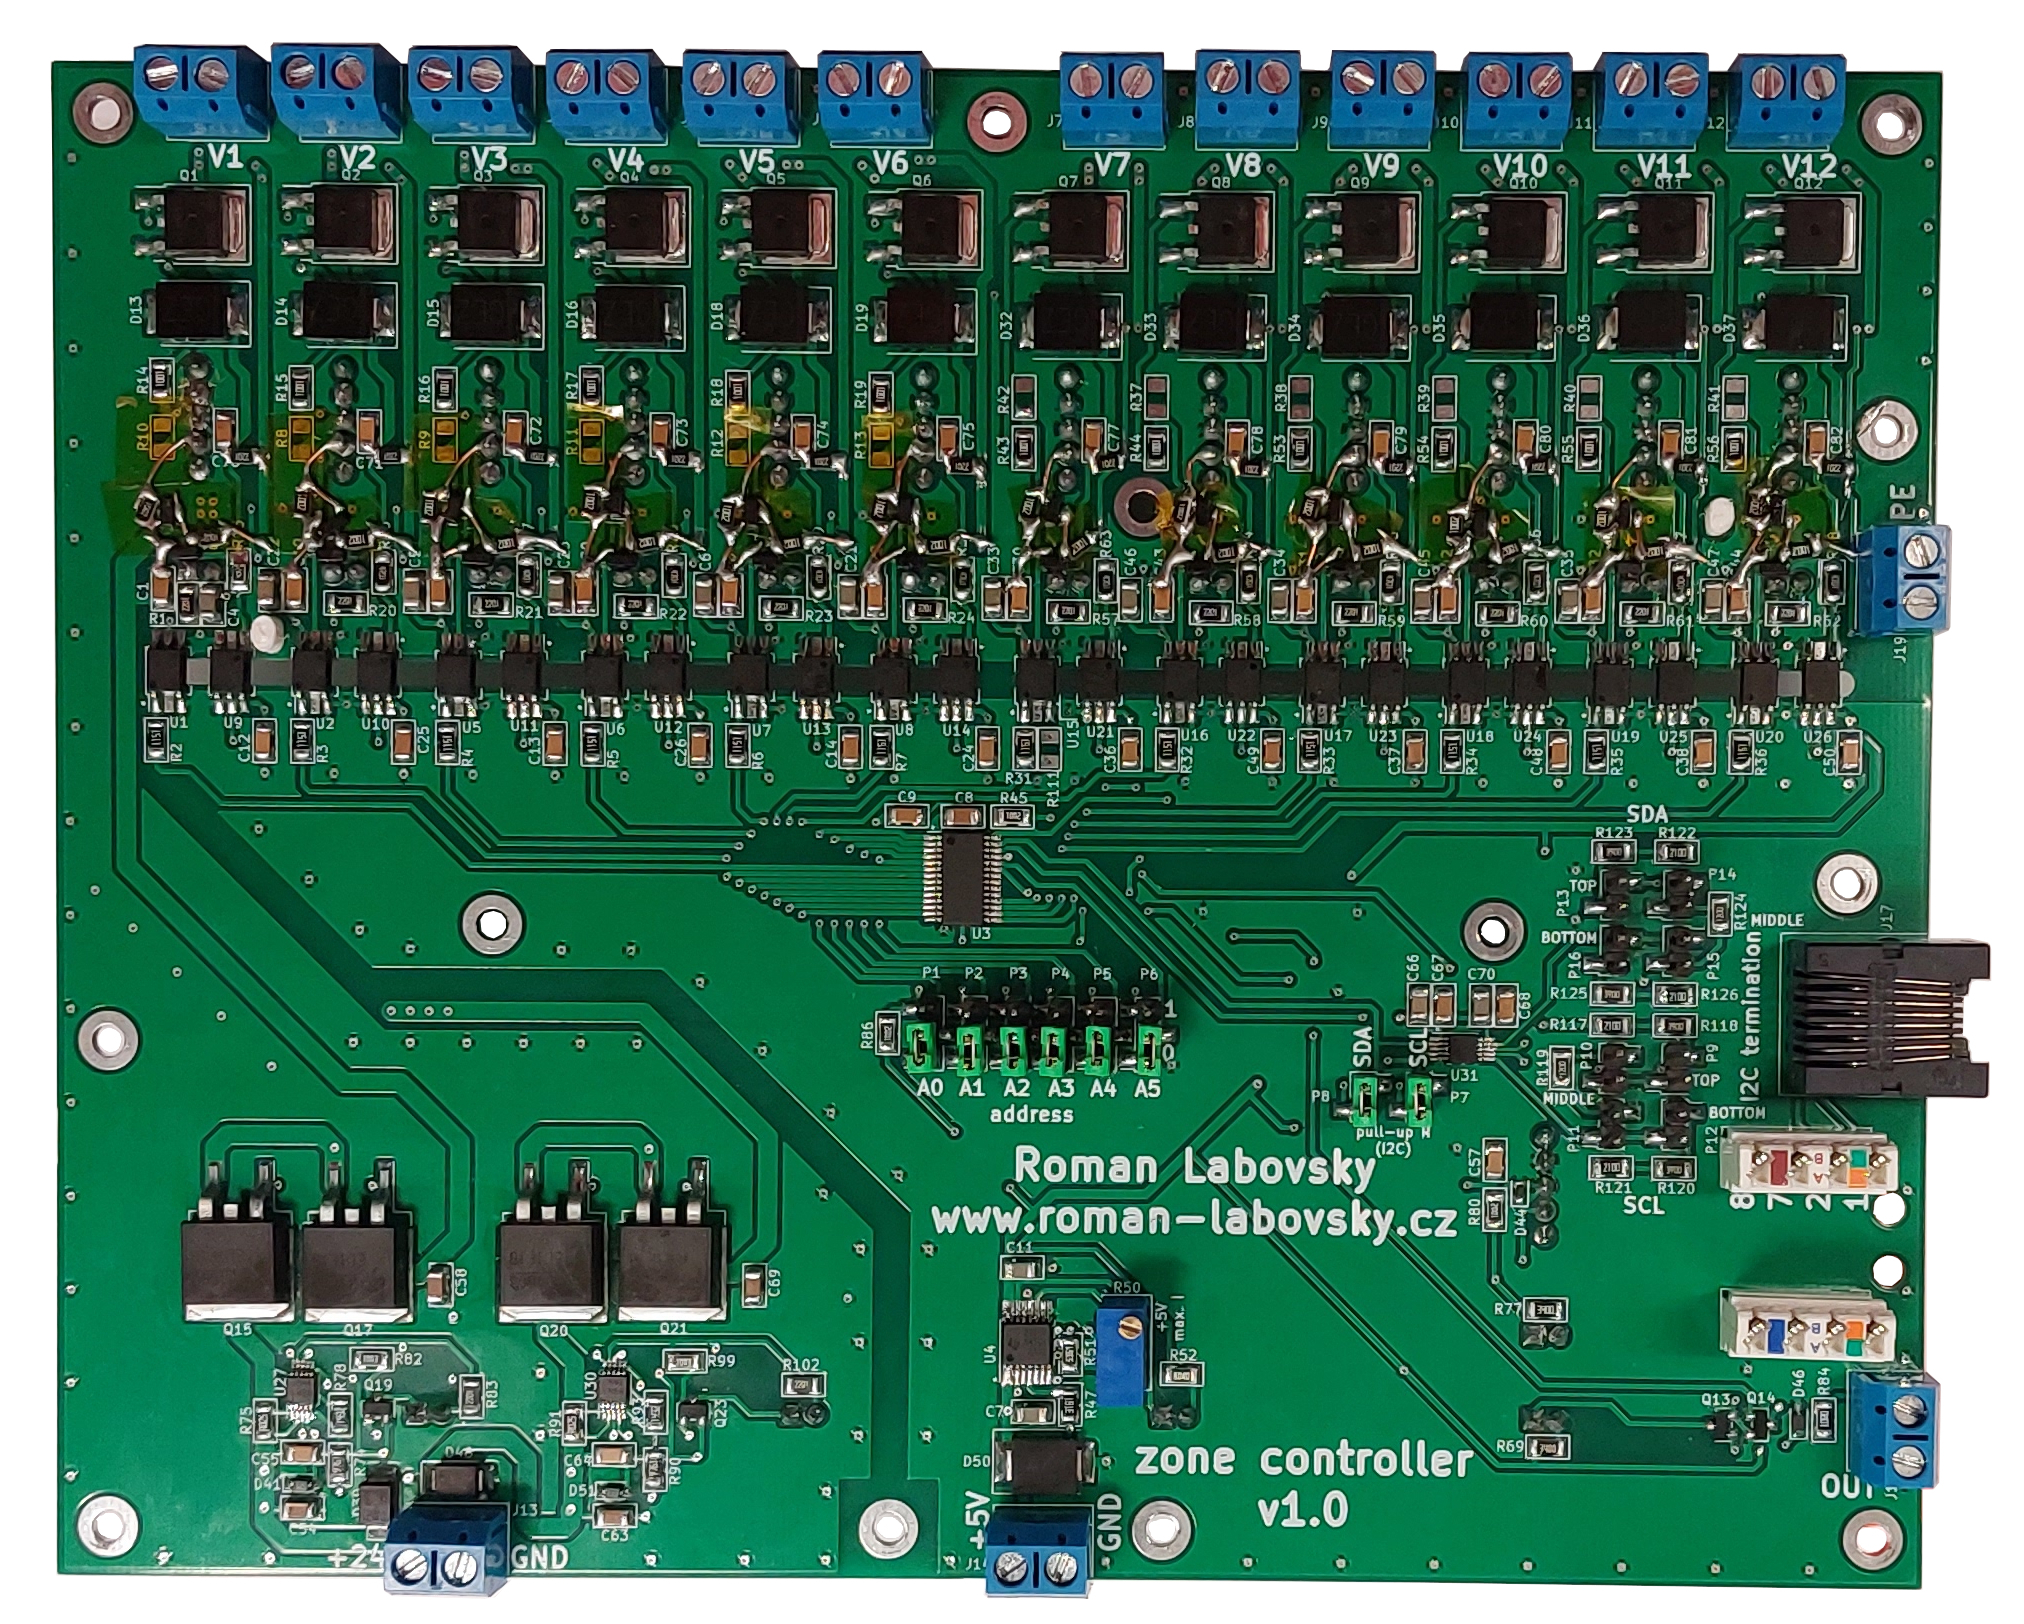
\includegraphics[width=\linewidth]{pictures/all/hardware/zone-controller-pcb-top.jpg}};
  
    \node[fill=black,text=white, draw=white] at (3.9,0.05) {1}; 
 	\node[fill=black,text=white, draw=white] at (9.25,0.05) {2};
    \node[fill=black,text=white, draw=white] at (17.5,1.6) {3};
    
    \node[fill=black,text=orange, draw=orange] at (16.1,3.3) {4}; 
    \draw[orange,line width=1mm,rounded corners] (15.2,2.2) rectangle (17,4.5);
    
    \node[fill=black,text=white, draw=white] at (17.5,5.4) {5};
    
    \node[fill=black,text=pink, draw=pink] at (7.5,5.1) {6}; 
    \draw[pink,line width=1mm,rounded corners] (7.8,4.2) rectangle (10.5,6);
    
    \node[fill=black,text=yellow, draw=yellow] at (13.7,5.5) {7}; 
    \draw[yellow,line width=1mm,rounded corners] (14.1,4) rectangle (15.2,7);
       
    \node[fill=black,text=white, draw=white] at (17.5,9.25) {8};
    
    \node[fill=black,text=red, draw=red] at (8.87,13.35) {9};
    \draw[red,line width=1mm,rounded corners] (1,12.5) rectangle (16.6,14.2);
\end{tikzpicture}
  \caption{The zone regulator. PCB}
  \label{fig:zone-controller-pcb-top}
\end{figure}
\end{English}

\begin{Czech}
\begin{figure}[H]
\centering
\begin{tikzpicture}[every text node part/.style={align=center}]
    \node[anchor=south west,inner sep=0] (image) at (0,0)   
   {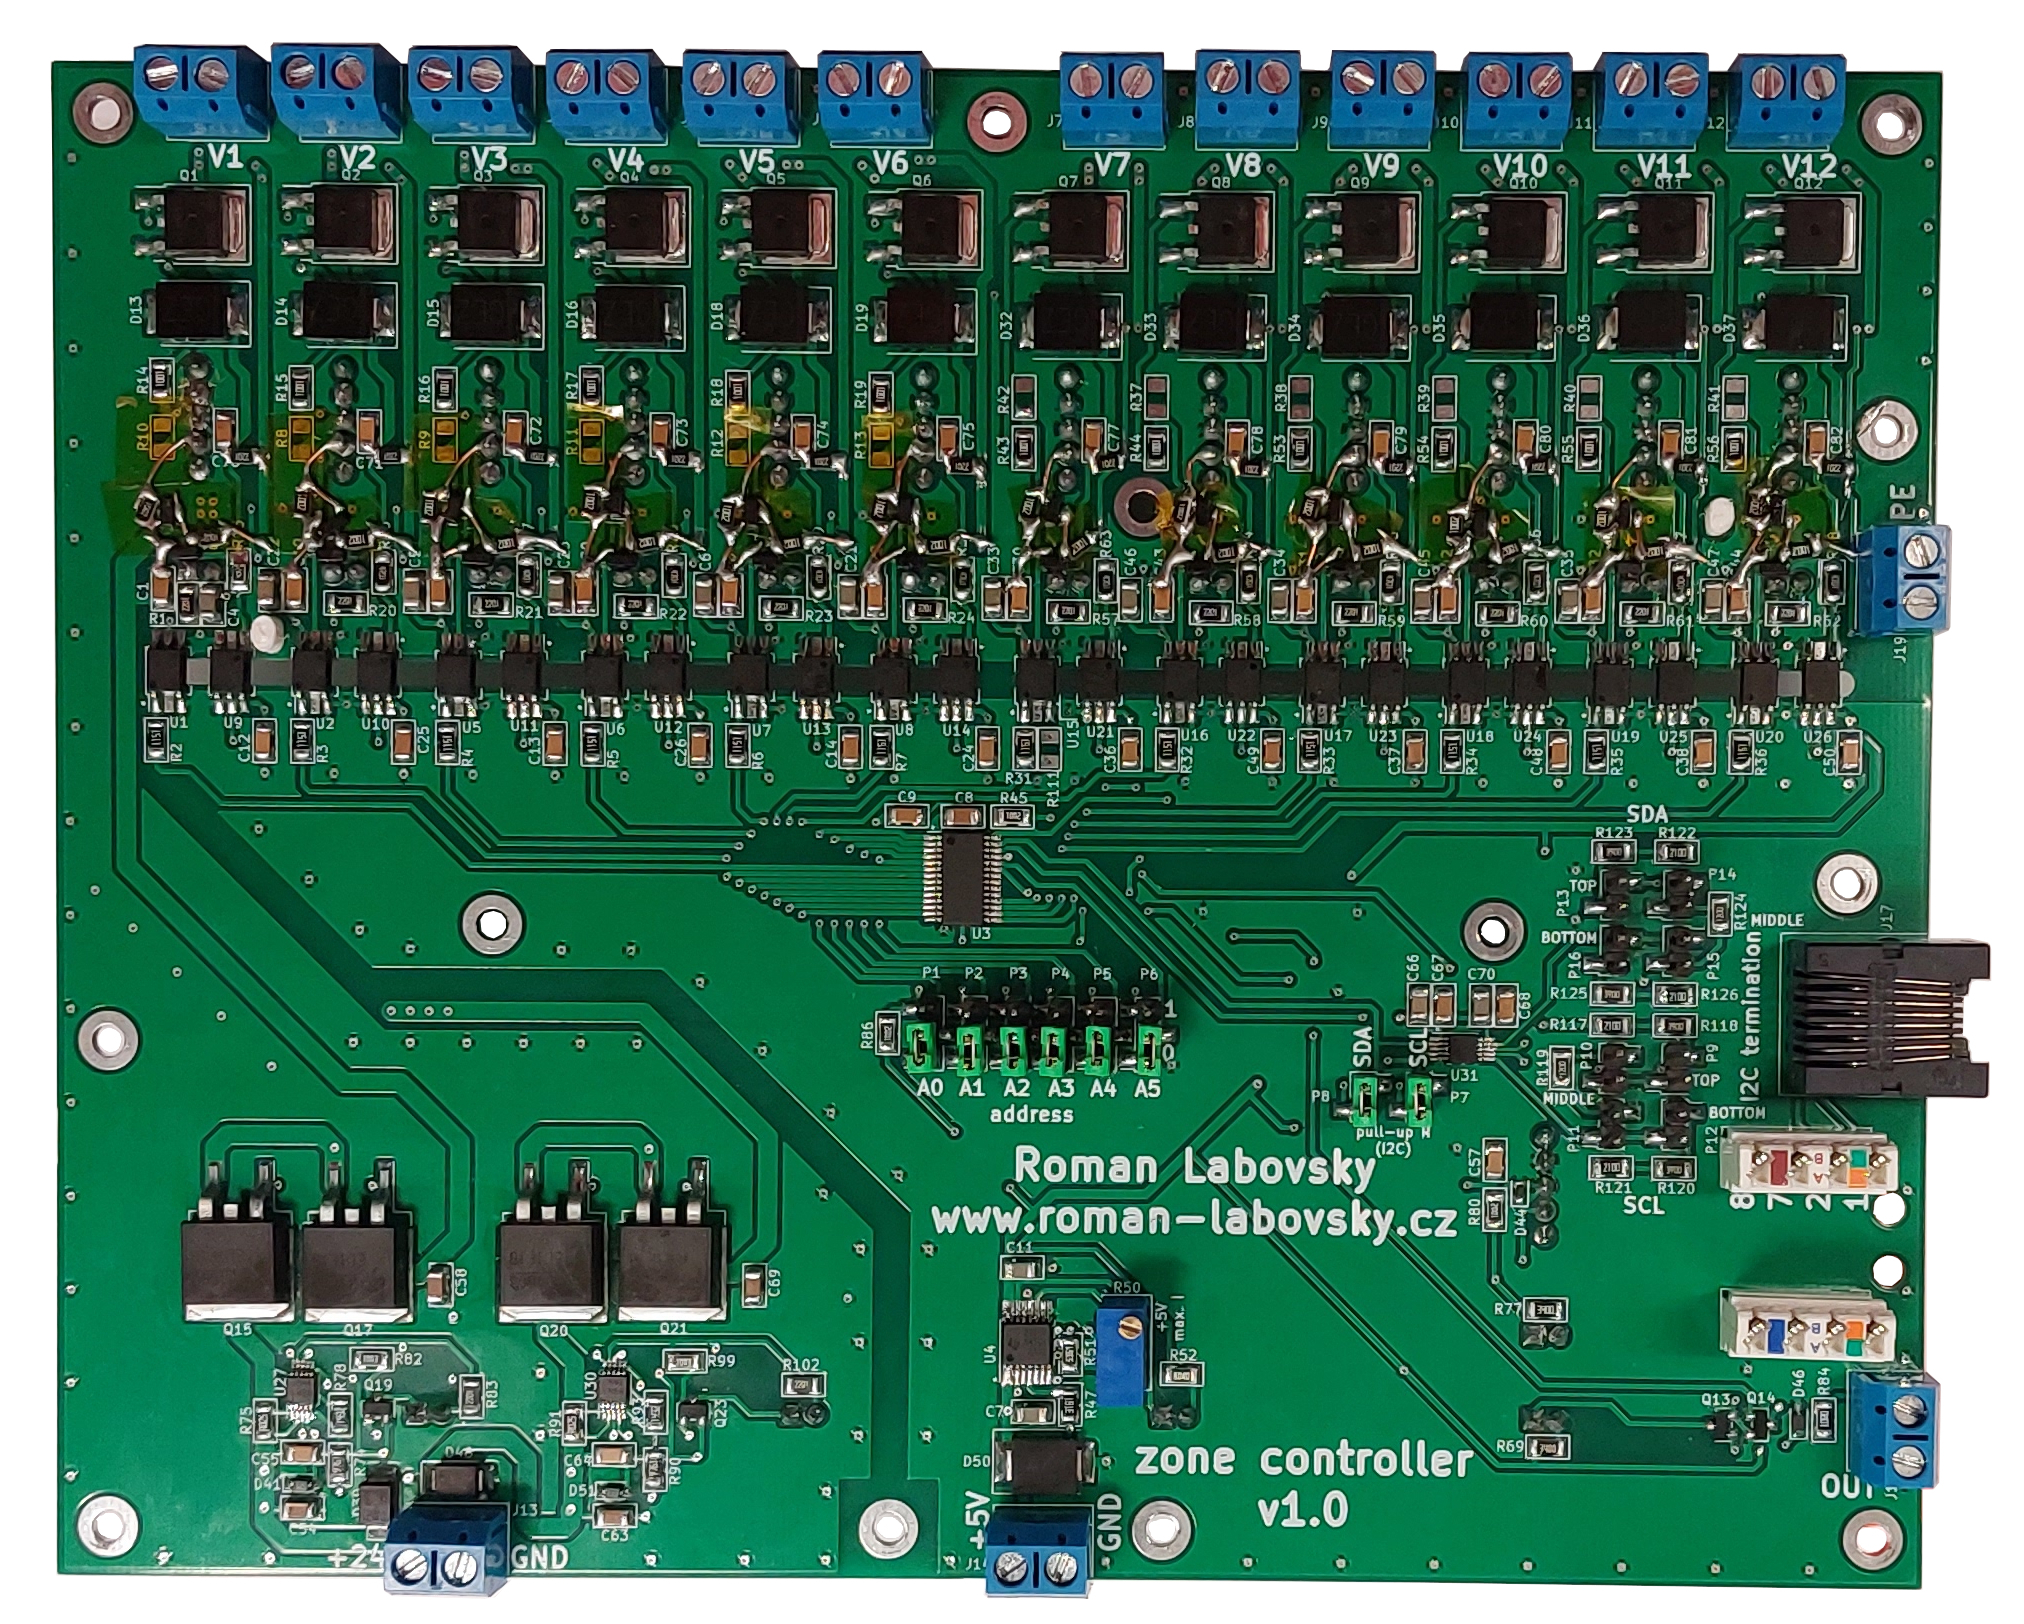
\includegraphics[width=\linewidth]{pictures/all/hardware/zone-controller-pcb-top.jpg}};
  
    \node[fill=black,text=white, draw=white] at (3.9,0.05) {1}; 
 	\node[fill=black,text=white, draw=white] at (9.25,0.05) {2};
    \node[fill=black,text=white, draw=white] at (17.5,1.6) {3};
    
    \node[fill=black,text=orange, draw=orange] at (16.1,3.3) {4}; 
    \draw[orange,line width=1mm,rounded corners] (15.2,2.2) rectangle (17,4.5);
    
    \node[fill=black,text=white, draw=white] at (17.5,5.4) {5};
    
    \node[fill=black,text=pink, draw=pink] at (7.5,5.1) {6}; 
    \draw[pink,line width=1mm,rounded corners] (7.8,4.2) rectangle (10.5,6);
    
    \node[fill=black,text=yellow, draw=yellow] at (13.7,5.5) {7}; 
    \draw[yellow,line width=1mm,rounded corners] (14.1,4) rectangle (15.2,7);
       
    \node[fill=black,text=white, draw=white] at (17.5,9.25) {8};
    
    \node[fill=black,text=red, draw=red] at (8.87,13.35) {9};
    \draw[red,line width=1mm,rounded corners] (1,12.5) rectangle (16.6,14.2);
\end{tikzpicture}
  \caption{Zónový regulátor. DPS}
  \label{fig:zone-controller-pcb-top}
\end{figure}
\end{Czech}


\begin{English}
\subsubsection{The Description of Marked Parts}
\end{English}

\begin{Czech}
\subsubsection{Popis označených částí}
\end{Czech}


\begin{English}
\subsubsubsection{The number 1}
Connector for connecting +24 V.
\end{English}

\begin{Czech}
\subsubsubsection{Číslo 1}
Konektor pro přípojení +24 V.
\end{Czech}


\begin{English}
\subsubsubsection{The number 2}
Connector for connecting +5 V.
\end{English}

\begin{Czech}
\subsubsubsection{Číslo 2}
Konektor pro přípojení +5 V.
\end{Czech}


\begin{English}
\subsubsubsection{The number 3}
Output connector for signaling (+5V (on) or 0V (off)) activation of the circulation pump. In case of manual activation of the circuit or pump.
\end{English}

\begin{Czech}
\subsubsubsection{Číslo 3}
Výstupní konektor pro signalizaci (+5 V (zapnuto) nebo 0 V (vypnuto)) zapnutí oběhového čerpadla. V případě manuálního zapnutí okruhu nebo čerpadla.
\end{Czech}


\begin{English}
\subsubsubsection{The number 4 \colorbox{Orange}{orange colour}}
The connector for connecting UTP cable or twisted pair without RJ45 connector using a punch-down tool. Input for I$^2$C bus. Same configuration as the number 5.
\end{English}

\begin{Czech}
\subsubsubsection{Číslo 4 \colorbox{Orange}{oranžová barva}}
Konektor pro připojení UTP kabelu respektive kroucené dvojlinky bez konektoru RJ45 pomocí narážejícího nástroje. Vstup I$^2$C sběrnice. Stejné zapojení jako u čísla 5.
\end{Czech}


\newpage
\begin{English}
\subsubsubsection{The number 5}
The connector for connecting UTP cable. Input for I$^2$C bus. Same configuration as the number 4.
\end{English}

\begin{Czech}
\subsubsubsection{Číslo 5}
Konektor pro připojení UTP kabelu. Vstup I$^2$C sběrnice. Stejné zapojení jako u čísla 4.
\end{Czech}


\begin{English}
\subsubsubsection{The number 6 \colorbox{CarnationPink}{pink colour}}
Jumpers for setting the device address for the I$^2$C bus. No need to reconfigure.
\end{English}

\begin{Czech}
\subsubsubsection{Číslo 6 \colorbox{CarnationPink}{růžová barva}}
Propojky na nastavení adresy zařízení pro I$^2$C sběrnici. Netřeba přenastavovat.
\end{Czech}


\begin{English}
\subsubsubsection{The number 7 \colorbox{Yellow}{yellow colour}}
Jumpers connect terminating resistors between wires for the I$^2$C bus. Enable only on devices with the longest UTP cable.
\end{English}

\begin{Czech}
\subsubsubsection{Číslo 7 \colorbox{Yellow}{žlutá barva}}
Propojky připojují ukončovací rezistory mezi vodiče pro I$^2$C sběrnici. Povolit pouze na zařízení s nejdelším UTP kabelem.
\end{Czech}


\begin{English}
\subsubsubsection{The number 8}
The connector for connecting the protective earth wire (PE).
\end{English}

\begin{Czech}
\subsubsubsection{Číslo 8}
Konektor pro připojení ochranného vodiče PE.
\end{Czech}


\begin{English}
\subsubsubsection{The number 9 \colorbox{Red}{red colour}}
Connectors for connecting thermoelectric valves to +24 V. The polarity connection is shown in the figure \ref{fig:zone-controller-terminal-block}. The orientation of the connector in the figure \ref{fig:zone-controller-terminal-block} is the same as the orientation in \ref{fig:zone-controller-pcb-top}.
\end{English}

\begin{Czech}
\subsubsubsection{Číslo 9 \colorbox{Red}{červená barva}}
Konektory pro připojení termoelektrický ventilů na +24 V. Připojení polarity je na obrázku \ref{fig:zone-controller-terminal-block}. Orientace konektoru na obrázku \ref{fig:zone-controller-terminal-block} je shodná s orientací na \ref{fig:zone-controller-pcb-top}.
\end{Czech}


\begin{English}
\begin{figure}[H]
    \centering
    \def\svgwidth{0.15\columnwidth}
    \graphicspath{{pictures/all/hardware/svg/}}
    \input{pictures/all/hardware/svg/zone-controller-terminal-block.pdf_tex}
    \caption{The connector for connecting the thermoelectric actuator. Similar marking is also present on the printed circuit board.}
    \label{fig:zone-controller-terminal-block}
\end{figure}
\end{English}

\begin{Czech}
\begin{figure}[H]
    \centering
    \def\svgwidth{0.15\columnwidth}
    \graphicspath{{pictures/all/hardware/svg/}}
    \input{pictures/all/hardware/svg/zone-controller-terminal-block.pdf_tex}
    \caption{Konektor pro připojení termoelektrického pohonu. Obdobné značení je i na desce plošných spojů.}
    \label{fig:zone-controller-terminal-block}
\end{figure}
\end{Czech}

% ====================  STOP Zone Controller ====================

\newpage
% ====================  START Wall-mounted Room Temperature Sensor ====================
\begin{English}
\subsection{Wall-mounted Room Temperature Sensor}
\end{English}

\begin{Czech}
\subsection{Nástěnný snímač prostorové teploty}
\end{Czech}


\begin{English}
In the figure \ref{fig:wall-mounted-room-temperature-sensor-with-case}, there is the wall-mounted room temperature sensor with a description of individual parts.
\end{English}

\begin{Czech}
Na obrázku \ref{fig:wall-mounted-room-temperature-sensor-with-case} je nástěnný snímač prostorové teploty s popisem jednotlivých částí.
\end{Czech}


\begin{Czech}
\begin{figure}[H]
\centering
\begin{tikzpicture}[font=\sffamily]
     \node[anchor=south west,inner sep=0] (image) at (0,0) {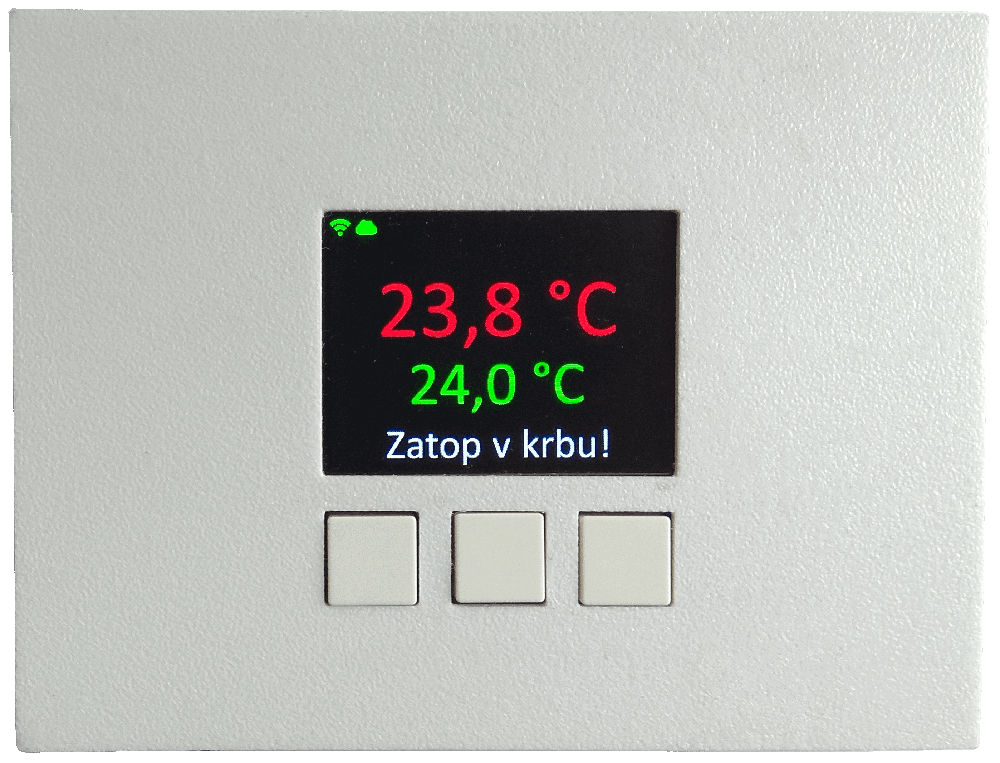
\includegraphics[width=0.9\textwidth]{pictures/all/hardware/wall-mounted-room-temperature-sensor-with-case.png}};
      \begin{scope}[x={(image.south east)},y={(image.north west)}]
     
     %   \draw[help lines,xstep=.1,ystep=.1] (0,0) grid (1,1);
    %    \foreach \x in {0,1,...,9} { \node [anchor=north] at (\x/10,0) {0.\x}; }
       % \foreach \y in {0,1,...,9} { \node [anchor=east] at (0,\y/10) {0.\y}; }
        
          \draw [red,-{Stealth[slant=0]}] (0.2,0.8)--(0.32,0.72);           
          \node[text=red] at (0.2,0.83) {Síťové připojení};
          
          \draw [red,{Stealth[slant=0]}-] (0.38,0.72)--(0.5,0.8);           
          \node[text=red] at (0.5,0.83) {Připojení k MQTT brokeru};
          
          \draw [red,-{Stealth[slant=0]}] (0.25,0.6)--(0.37,0.6);
          \node[text=red] at (0.12,0.6) {Aktuální teplota};
          
          \draw [red,{Stealth[slant=0]}-] (0.6,0.5)--(0.72,0.5);
          \node[text=red] at (0.9,0.5) {Požadovaná teplota};
          
          \draw [red,-{Stealth[slant=0]}] (0.25,0.42)--(0.37,0.42);
          \node[text=red] at (0.12,0.42) {Zpráva uživateli};
          
          \draw [red,-{Stealth[slant=0]}] (0.25,0.26)--(0.37,0.26);
          \node[text=red] at (0.1,0.28) {Dekrementování};
          \node[text=red] at (0.1,0.23) {požadované teploty};
          
          \draw [red,{Stealth[slant=0]}-] (0.62,0.26)--(0.74,0.26);
          \node[text=red] at (0.9,0.28) {Inkrementování};
          \node[text=red] at (0.9,0.23) {požadované teploty};
          
          \draw [red,{Stealth[slant=0]}-] (0.5,0.26)--(0.6,0.1);
          \node[text=red] at (0.65,0.1) {Menu};
        \end{scope}
\end{tikzpicture}
\caption{Nástěnný snímač prostorové teploty.}
\label{fig:wall-mounted-room-temperature-sensor-with-case}
\end{figure}
\end{Czech}

\begin{Czech}
Ikona síťového přípojení signalizuje stav k připojení na kabel nebo WiFi. Ikona přípojení k MQTT brokeru značí stav připojení k centrální jednotce (stav připojení je též signalizován na příslušném termostatu v systému). Zelená barva značí stav připojeno, červená ikona stav odpojeno. Tlačítko menu v současné době neobsahuje žádnou funkcionalitu. V  případě, že bude požadavek na zatopení v krbu, též signalizace pomocí modré LED (viz část \ref{sec:} „\textit{LED indikace – mezní parametry zásobníku teplé vody}“) jsou uživatelé na všech nástěnných snímačích prostorové tepoty o této skutečnosti informováni. Obdobná informace se též zobrazuje na všech displejích u LED indikace.
\end{Czech}

% ====================  STOP Wall-mounted room temperature sensor ====================

\begin{Czech}
\subsection{Signalizace u krbu}
\end{Czech}

\begin{Czech}
Na obrázku \ref{fig:signalization-by-fireplace-case-top} je signalizace s popisem jednotlivých částí.
\end{Czech}

\begin{Czech}
\begin{figure}[H]
\centering
\begin{tikzpicture}[every text node part/.style={align=center}]
    \node[anchor=south west,inner sep=0] (image) at (0,0)   
   {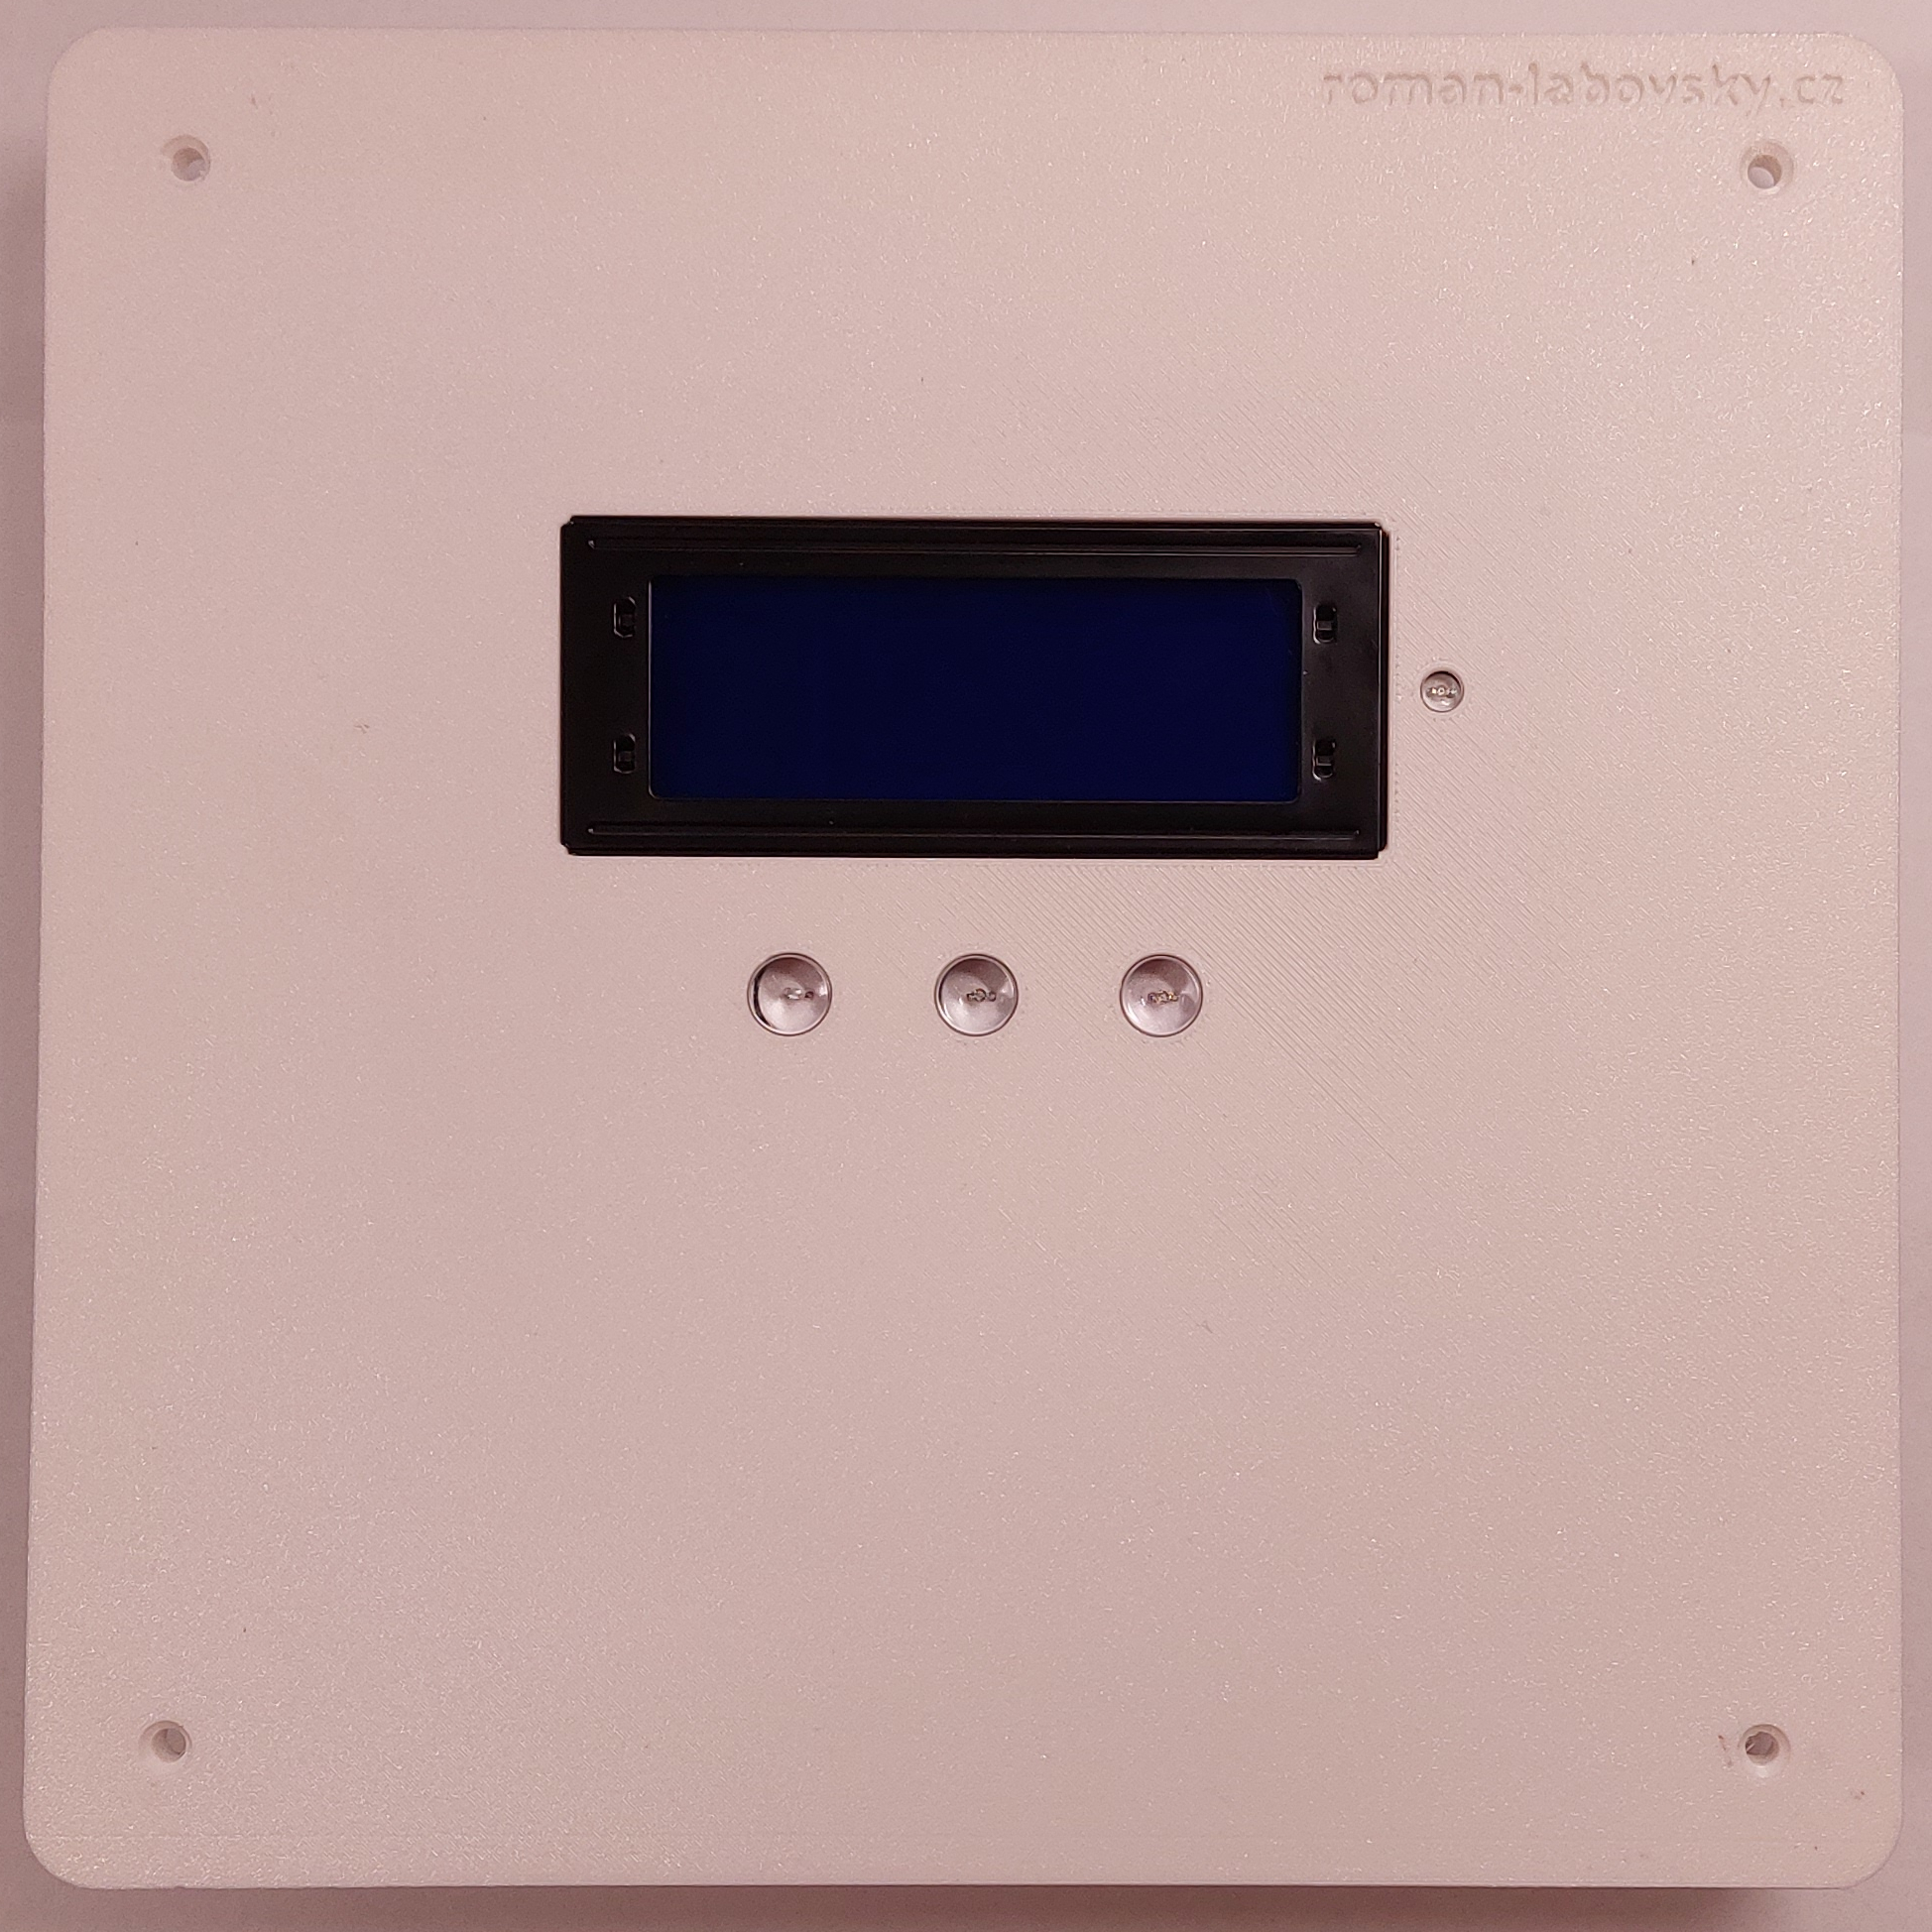
\includegraphics[width=\linewidth]{pictures/all/hardware/signalization-by-fireplace-case-top.jpg}};
  
    \node[text=red] at (9,13.5) {1}; 
    \node[text=red] at (13.45,12) {2};    
    \node[text=red] at (7.35,9.5) {3};   
    \node[text=red] at (9.1,9.5) {4};   
    \node[text=red] at (10.85,9.5) {5};              
\end{tikzpicture}
  \caption{Signalizace u krbu. Vrchní část s panelem.}
  \label{fig:signalization-by-fireplace-case-top}
\end{figure}
\end{Czech}

\begin{Czech}
\subsubsection{Popis označených částí}
\end{Czech}

\begin{Czech}
\subsubsubsection{Číslo 1}
Displej pro zobrazování teploty v zásobníku otopné vody ve všech 3 částí. Spodní řádek displeje může zobrazovat zprávy uživatelům.
\end{Czech}

\begin{Czech}
\subsubsubsection{Číslo 2}
Signalizační LED pro +5 V. Pokud bliká je aktivovaná nadproudová ochrana.
\end{Czech}

\newpage
\begin{Czech}
\subsubsubsection{Číslo 3}
Signalizační modrá LED. Pokud LED svítí, tak horní část zásobníku otopné vody není dostatečně nahřátá, teplota je nižší než nastavená mez. Softwarové nastavení spínání je v části \ref{sec:led-indication} \textit{LED indikace – mezní parametry zásobníku teplé vody}.
\end{Czech}

\begin{Czech}
\subsubsubsection{Číslo 4}
Signalizační oranžová LED. Pokud LED svítí, tak střední část zásobníku otopné vody je dostatečně nahřátá, teplota je rovna nebo vyšší než nastavená mez. Softwarové nastavení spínání je v části \ref{sec:led-indication} \textit{LED indikace – mezní parametry zásobníku teplé vody}.
\end{Czech}

\begin{Czech}
\subsubsubsection{Číslo 5}
Signalizační červená LED. Pokud LED svítí, tak spodní část zásobníku otopné vody je dostatečně nahřátá, teplota je rovna nebo vyšší než nastavená mez. Softwarové nastavení spínání je v části \ref{sec:led-indication} \textit{LED indikace – mezní parametry zásobníku teplé vody}.
\end{Czech}

\begin{Czech}
\begin{figure}[H]
\centering
\begin{tikzpicture}[every text node part/.style={align=center}]
    \node[anchor=south west,inner sep=0] (image) at (0,0)   
   {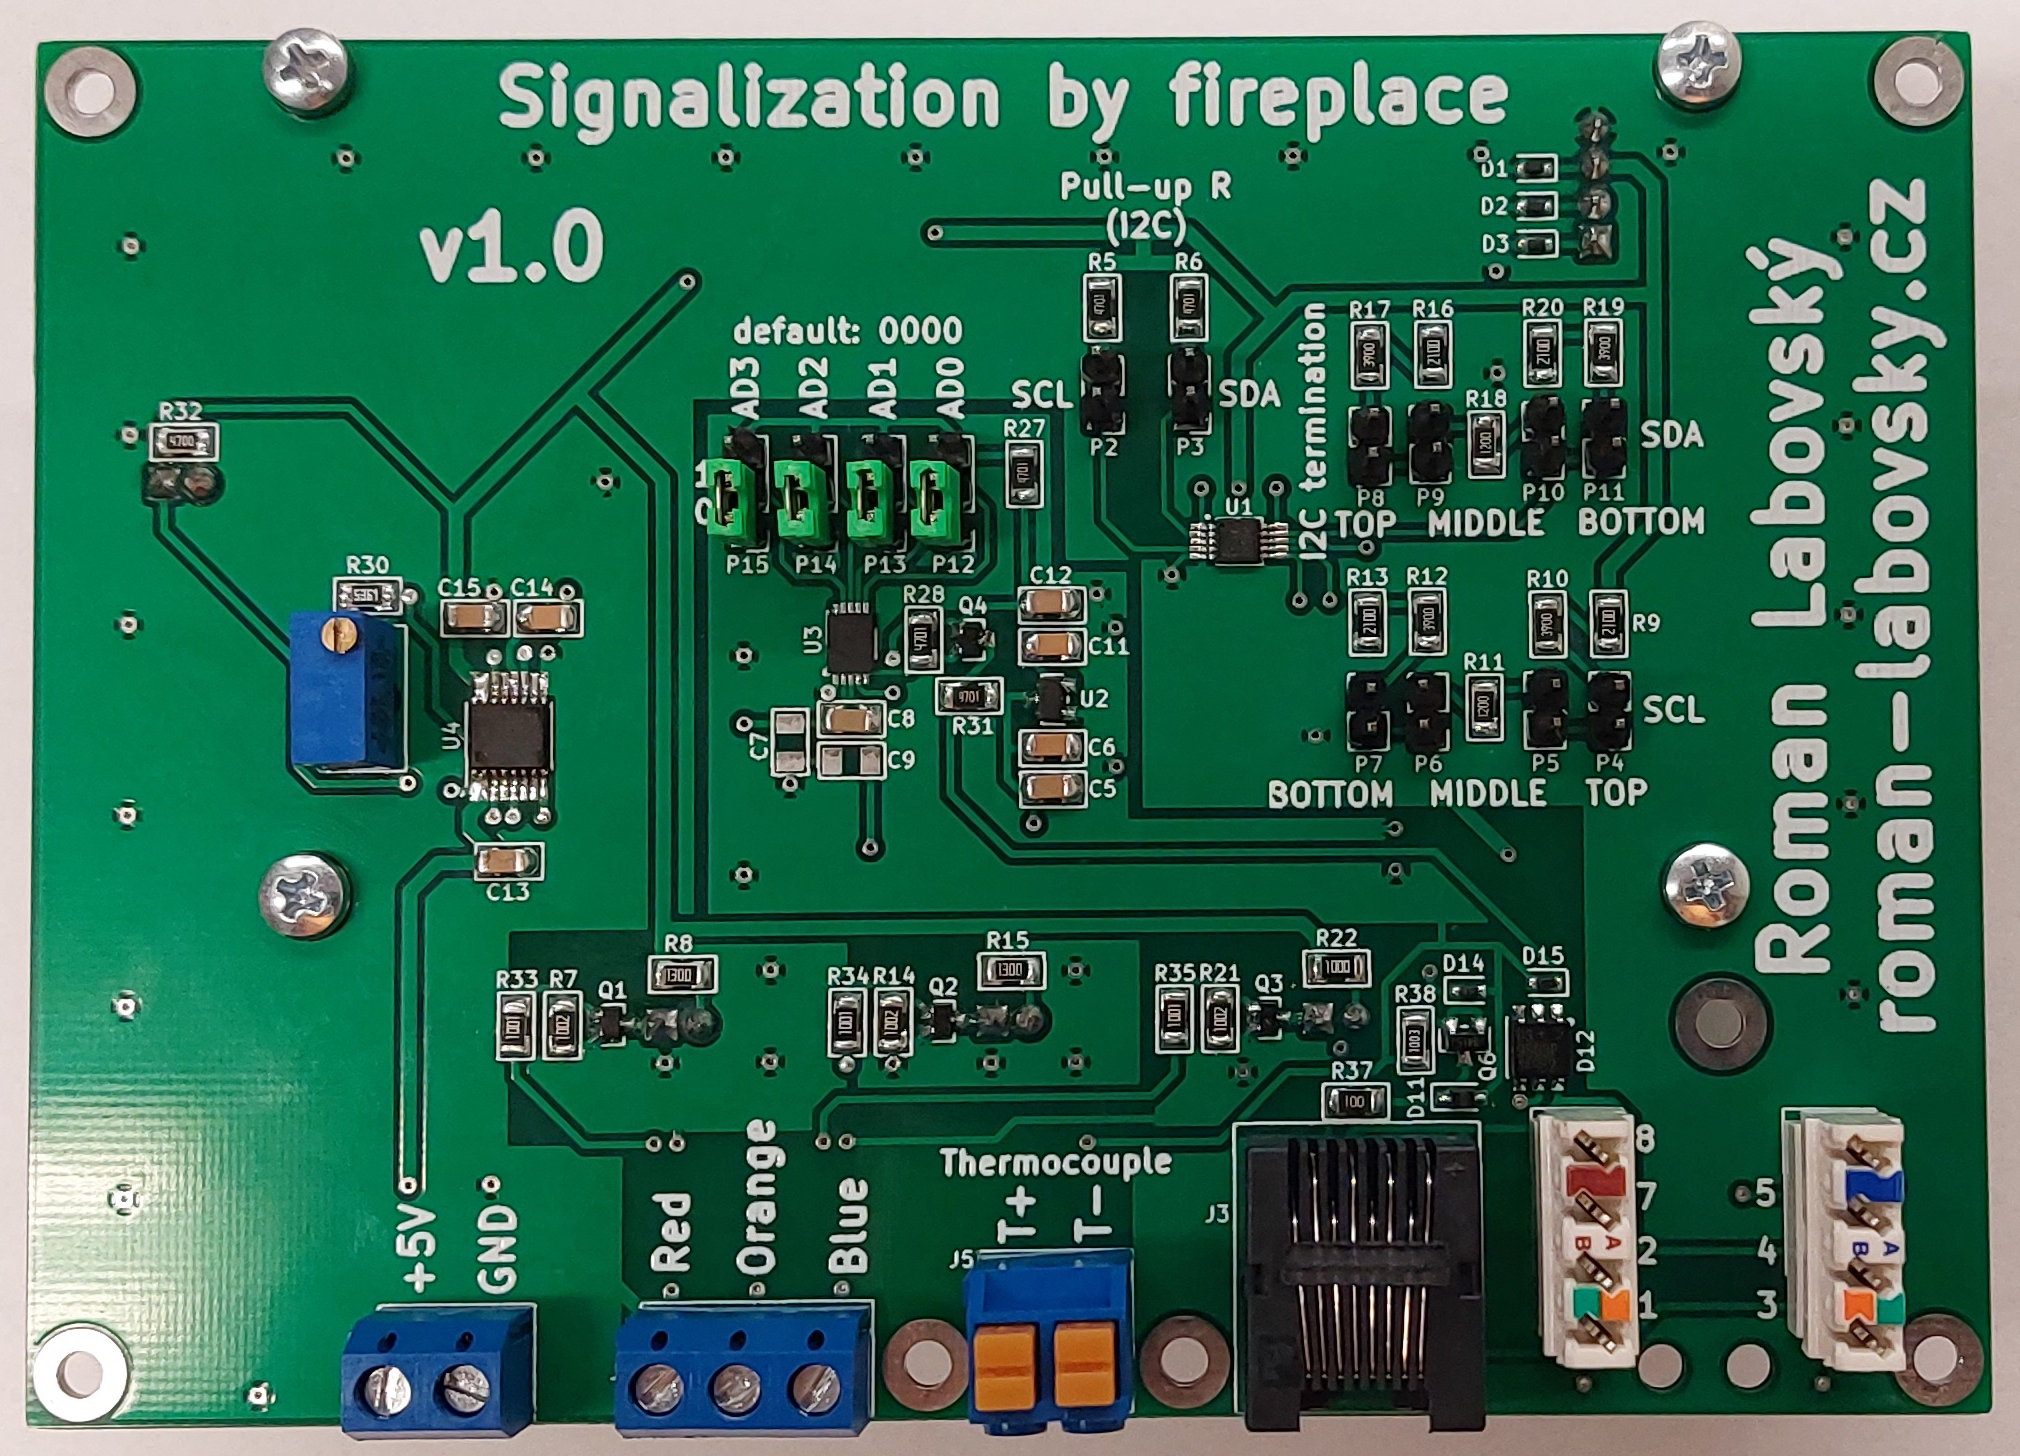
\includegraphics[width=\linewidth]{pictures/all/hardware/signalization-by-fireplace-pcb-top.jpg}};
  
    \node[fill=black,text=white, draw=white] at (3.8,0.0) {1}; 
 	\node[fill=black,text=white, draw=white] at (6.65,0.0) {2};
    \node[fill=black,text=white, draw=white] at (9.45,0.0) {3};
    \node[fill=black,text=white, draw=white] at (12.15,0.0) {4};
    \node[fill=black,text=white, draw=white] at (15.35,0.0) {5};
    
    \node[fill=black,text=orange, draw=orange] at (3,8.1) {6}; 
    \draw[orange,line width=1mm,rounded corners] (2.5,6) rectangle (3.5,7.7);
    
    \node[fill=black,text=pink, draw=pink] at (5.6,8.5) {7}; 
    \draw[pink,line width=1mm,rounded corners] (6,8) rectangle (9,9);
    
    \node[fill=black,text=yellow, draw=yellow] at (10.2,10.4) {8}; 
    \draw[yellow,line width=1mm,rounded corners] (9.4,9) rectangle (11,10);
    
    \node[fill=black,text=red, draw=red] at (13.25,8) {9};
    \draw[red,line width=1mm,rounded corners] (11.9,6) rectangle (14.7,9.8);
\end{tikzpicture}
  \caption{Signalizace u krbu. DPS.}
  \label{fig:signalization-by-fireplace-pcb-top}
\end{figure}
\end{Czech}

\begin{Czech}
\subsubsection{Popis označených částí}
\end{Czech}

\begin{Czech}
\subsubsubsection{Číslo 1}
Konektor pro přípojení +5 V.
\end{Czech}

\begin{Czech}
\subsubsubsection{Číslo 2}
Konektor pro kabelů pro signalizačních kabelů modré, oranžové a červené LED.
\end{Czech}

\begin{Czech}
\subsubsubsection{Číslo 3}
Konektor pro připojení termočlánku. Dodržet polaritu.
\end{Czech}

\begin{Czech}
\subsubsubsection{Číslo 4}
Konektor pro UTP kabelu. Vstup I$^2$C sběrnice a 1-Wire sběrnice. Stejné zapojení jako u čísla 5.
\end{Czech}

\begin{Czech}
\subsubsubsection{Číslo 5}
Konektor pro UTP kabelu respektive kroucené dvojlinky bez konektory RJ45 pomocí narážejícího nástroje. Vstup I$^2$C sběrnice a 1-Wire sběrnice. Stejné zapojení jako u čísla 4. Čísla označují vodiče (pořadí) v UTP kabelu.
\end{Czech}

\begin{Czech}
\subsubsubsection{Číslo 6  \colorbox{Orange}{oranžová barva}}
Trimer pro nastavení maximálního proudu pro +5 V. Netřeba přenastavovat.
\end{Czech}

\begin{Czech}
\subsubsubsection{Číslo 7  \colorbox{CarnationPink}{růžová barva}}
Propojky pro nastavení adresy zařízení pro 1-Wire sběrnici. Netřeba přenastavovat. Nechat na 0000.
\end{Czech}

\begin{Czech}
\subsubsubsection{Číslo 8  \colorbox{Yellow}{žlutá barva}}
Propojky pro nastavení pull-up rezistorů pro I$^2$C sběrnici. Netřeba přenastavovat.
\end{Czech}

\begin{Czech}
\subsubsubsection{Číslo 9 \colorbox{Red}{červená barva}}
Propojky připojují ukončovací rezistory mezi vodiče I$^2$C sběrnici. Povolit pouze na zařízení s nejdelším UTP kabelem.
\end{Czech}

% ========================================

\begin{Czech}
\subsection{Adresy/ID zařízení a další}
\end{Czech}

\begin{Czech}
\subsubsection{I$^2$C sběrnice}
\end{Czech}

\begin{Czech}
V tabulce \ref{tab:i2c-bus-signalizations} jsou vidět jednotlivé adresy pro signalizace u krbů (displeje) na I$^2$C sběrnici. Propojky A3, A2, A1 je nutné mít stejně na zařízeních nastavené. Propojky se nacházejí na zadní straně displeje. Pro nastavení logické 0 je nutné vložit propojku.
\end{Czech}

\begin{Czech}
\begin{table}[H]
\centering
\begin{tabular}{||c || c c c c||} 
 \hline
 Adresa I$^2$C & Centrální jednotka & Signalizace – sklep & Signalizace – přízemí & Signalizace – patro \\  
 \hline\hline
  A3 A2 A1 & 011 & 101 & 111 & 110 \\ 
 \hline
\end{tabular}
\caption{Nastavení adres pro signalizace (displeje) na I$^2$C sběrnici.}
\label{tab:i2c-bus-signalizations}
\end{table}
\end{Czech}

\begin{Czech}
V tabulce \ref{tab:i2c-bus-zone-controllers} jsou vidět jednotlivé adresy pro zónové regulátorů  v rozdělovačích na I$^2$C sběrnici. Propojky A5, A4, A3, A2, A1, A0 je nutné mít stejně na zařízeních nastavené. Propojky se nacházejí na zadní straně DPS podle obrázku \ref{fig:zone-controller-pcb-top} v růžovém obdélníku. Pro nastavení logické 0 je nutné vložit propojku dolu, pro logickou 1 je nutné vložit propojku nahoru.
\end{Czech}

\begin{Czech}
\begin{table}[H]
\centering
\begin{tabular}{||c || c c ||} 
 \hline
 Adresa I$^2$C & Rozdělovač  – přízemí & Rozdělovač  – patro \\ 
 \hline\hline
 A5 A4 A3 A2 A1 A0 & 000 001 & 000 000\\ 
 \hline
\end{tabular}
\caption{Nastavení adres pro zónové regulátory v rozdělovačích na I$^2$C sběrnici.}
\label{tab:i2c-bus-zone-controllers}
\end{table}
\end{Czech}

\begin{Czech}
Zakončovací rezistory na I$^2$C sběrnici jsou na straně centrální jednotky (rozvaděč) a na signalizaci u krbu v patře.
\end{Czech}

% ========================================

\begin{Czech}
\subsubsection{1-Wire sběrnice}
\end{Czech}

\begin{Czech}
V tabulce \ref{tab:1-wire-bus} jsou místa a ID teplotních senzorů na 1-Wire sběrnici.
\end{Czech}

\begin{Czech}
\begin{table}[H]
\centering
\begin{tabular}{|c| c ||} 
 \hline
  Místo & ID senzoru \\ 
 \hline\hline
 Kouřovod – krb sklep & 3b-4c74109d6361 \\ 
 Kouřovod – krb přízemí & 3b-4c74109d636d \\ 
 Kouřovod – krb patro & 3b-4c74109d6349\\ 
 Zásobník otopné vody – spodek & 28-00000c864409 \\ 
 Zásobník otopné vody – střed & 28-00000c85a5bc \\ 
 Zásobník otopné vody – vršek & 28-00000c859e14 \\ 
 Venkovní senzor & 28-00000c85a20f \\ 
 \hline
\end{tabular}
\caption{ID teplotních senzorů 1-Wire sběrnice.}
\label{tab:1-wire-bus}
\end{table}
\end{Czech}